\documentclass[10pt,a4paper]{article}
\usepackage[utf8]{inputenc}
\usepackage{amsmath}
\usepackage{amsfonts}
\usepackage{amssymb}
\usepackage{amsthm}
\usepackage{float}
\usepackage{mathtools}
\usepackage{geometry}[margin=1in]
\usepackage{xspace}
\usepackage{tikz}
\usepackage{mathrsfs}
\usetikzlibrary{shapes, arrows, decorations.pathmorphing, ducks, automata}
\usepackage[parfill]{parskip}
\usepackage{subcaption}
\usepackage{stmaryrd}
\usepackage{marvosym}
\usepackage{dsfont}
\usepackage{centernot}

\setlength{\parindent}{1em}

\newcommand{\st}{\text{ s.t. }}
\newcommand{\contr}{\lightning}
\newcommand{\im}{\mathfrak{i}}
\newcommand{\R}{\mathbb{R}}
\newcommand{\Q}{\mathbb{Q}}
\newcommand{\C}{\mathbb{C}}
\newcommand{\F}{\mathbb{F}}
\newcommand{\K}{\mathbb{K}}
\newcommand{\N}{\mathbb{N}}
\newcommand{\Z}{\mathbb{Z}}
\newcommand{\E}{\mathbb{E}}
\renewcommand{\P}{\mathbb{P}}
\renewcommand{\H}{\mathds{H}}
\newcommand{\nequiv}{\not\equiv}
\newcommand{\powset}{\mathcal{P}}
\renewcommand{\th}[1][th]{\textsuperscript{#1}\xspace}
\newcommand{\from}{\leftarrow}
\newcommand{\legendre}[2]{\left(\frac{#1}{#2}\right)}
\newcommand{\ow}{\text{otherwise}}
\newcommand{\imp}[2]{\underline{\textit{#1.}$\implies$\textit{#2.}}}
\let\oldexists\exists
\renewcommand{\exists}{\oldexists\;}
\renewcommand{\hat}{\widehat}
\renewcommand{\tilde}{\widetilde}
\newcommand{\one}{\mathds{1}}
\newcommand{\under}{\backslash}
\newcommand{\injection}{\hookrightarrow}
\newcommand{\surjection}{\twoheadrightarrow}
\newcommand{\jacobi}{\legendre}
\newcommand{\floor}[1]{\lfloor #1 \rfloor}
\newcommand{\ceil}[1]{\lceil #1 \rceil}
\newcommand{\cbrt}[1]{\sqrt[3]{#1}}
\renewcommand{\angle}[1]{\langle #1 \rangle}
\renewcommand{\o}{\mathfrak{o}}
\newcommand{\dbangle}[1]{\angle{\angle{#1}}}
\newcommand{\false}{\textsc{False}}
\newcommand{\taut}{\vDash}
\newcommand{\ket}[1]{|#1\rangle}
\newcommand{\bra}[1]{\langle #1|}
\newcommand{\braket}[2]{\langle #1 | #2 \rangle}
\newcommand{\colvec}[1]{\begin{pmatrix} #1 \end{pmatrix}}

\DeclareMathOperator{\ex}{ex}
\DeclareMathOperator{\id}{id}
\DeclareMathOperator{\upper}{Upper}
\DeclareMathOperator{\dom}{dom}
\DeclareMathOperator{\disc}{disc}
\DeclareMathOperator{\charr}{char}
\DeclareMathOperator{\Image}{im}
\DeclareMathOperator{\ord}{ord}
\DeclareMathOperator{\lcm}{lcm}
\DeclareMathOperator{\aut}{Aut}
\DeclareMathOperator{\diag}{diag}
\DeclareMathOperator{\stab}{stab}
\DeclareMathOperator{\trace}{trace}
\DeclareMathOperator{\ecl}{ecl}
\DeclareMathOperator{\Span}{Span}
\DeclareMathOperator{\Gal}{Gal}
\DeclareMathOperator{\Var}{Var}
\let\Re\relax
\let\Im\relax
\DeclareMathOperator{\Re}{\mathfrak{Re}}
\DeclareMathOperator{\Im}{\mathfrak{Im}}
\DeclareMathOperator{\Frac}{Frac}

\let\emph\relax
\DeclareTextFontCommand{\emph}{\bfseries\em}

\newtheorem{theorem}{Theorem}[section]
\newtheorem{lemma}[theorem]{Lemma}
\newtheorem{corollary}[theorem]{Corollary}
\newtheorem{proposition}[theorem]{Proposition}
\newtheorem{conjecture}[theorem]{Conjecture}

\tikzset{sketch/.style={decorate,
 decoration={random steps, amplitude=1pt, segment length=5pt}, 
 line join=round, draw=black!80, very thick, fill=#1
}}

\title{Algebraic Topology}
\begin{document}
\maketitle

\section{Introduction}
The fundamental problem of topology is to establish whether or not there exist continuous functions $f, g$ going from a topological space $X$ to another space $Y$ and back again. For example, in the case of this torus and double-torus, we know from Geometry that such functions cannot exist by considering the Euler characteristic, but in general this is a hard problem.
\begin{center}
\scalebox{0.9}{
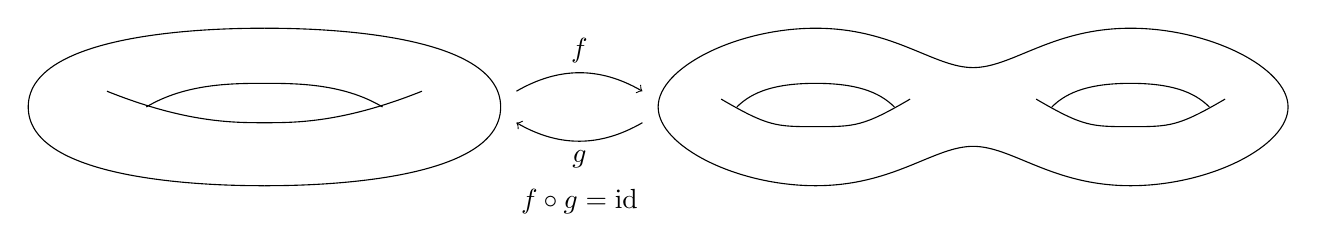
\begin{tikzpicture}
\draw (-7,0) .. controls (-7,1) and (-4.4,1) .. (-4,1);
\draw (-7,0) .. controls (-7,-1) and (-4.4,-1) .. (-4,-1);
\draw (-1,0) .. controls (-1,1) and (-3.6,1) .. (-4,1);
\draw (-1,0) .. controls (-1,-1) and (-3.6,-1) .. (-4,-1);
\draw (-5.5,0) .. controls (-5,0.3) and (-4.4,0.3) .. (-4,0.3) .. controls (-3.6,0.3) and (-3,0.3) .. (-2.5,0);
\draw (-6,0.2) .. controls (-5,-0.2) and (-4.4,-0.2) .. (-4,-0.2) .. controls (-3.6,-0.2) and (-3,-0.2) .. (-2,0.2);

\draw (1,0) .. controls (1,0.5) and (2,1) .. (3,1) .. controls (4,1) and (4.5,0.5) .. (5,0.5) .. controls (5.5,0.5) and (6,1) .. (7,1) .. controls (8,1) and (9,0.5) .. (9,0);
\draw (1,0) .. controls (1,-0.5) and (2,-1) .. (3,-1) .. controls (4,-1) and (4.5,-0.5) .. (5,-0.5) .. controls (5.5,-0.5) and (6,-1) .. (7,-1) .. controls (8,-1) and (9,-0.5) .. (9,0);
\draw (2,0) .. controls (2.2,0.2) and (2.5,0.3) .. (3,0.3) .. controls (3.5,0.3) and (3.8,0.2) .. (4,0);
\draw (1.8,0.1) .. controls (2.4,-0.25) and (2.5,-0.25) .. (3,-0.25) .. controls (3.5,-0.25) and (3.6, -0.25) .. (4.2,0.1);
\draw (6,0) .. controls (6.2,0.2) and (6.5,0.3) .. (7,0.3) .. controls (7.5,0.3) and (7.8,0.2) .. (8,0);
\draw (5.8,0.1) .. controls (6.4,-0.25) and (6.5,-0.25) .. (7,-0.25) .. controls (7.5,-0.25) and (7.6, -0.25) .. (8.2,0.1);

\draw (-0.8,0.2) edge[bend left, ->] node[above] {$f$} (0.8,0.2);
\draw (0.8,-0.2) edge[bend left, ->] node[below] {$g$} (-0.8,-0.2);
\node at (0,-1.2) {$f \circ g = \id$};
\end{tikzpicture}}
\end{center}
If such $f, g$ continuous functions exist, then we say the two spaces are homeomorphic. Basic idea of algebraic topology is that we want to associate to any topological space $X$ a group $G(X)$, and for every continuous function $f:X \rightarrow Y$ a group homomorphism $G(f): G(X) \rightarrow G(Y)$ with $G(\id) = \id$ and $G(f\circ g)=G(f)\circ G(g)$. Thus if $f:X\rightarrow Y$ is a homeomorphism with inverse $g:Y\rightarrow X$, then $G(g)\circ G(f)=\id, G(f)\circ G(g) = \id$, so $G(f)$ is an is an isomorphism.

\underline{Extension problem:} Let $X$ be a topological space, $A\subseteq X$ a subspace, and $f:A\rightarrow Y$ a continuous function. Does there exist a continuous function $F:X\rightarrow Y$ with $F|_A = f$
\begin{center}
\tikz{
\node (A) at (0,0) [circle] {$A$};
\node (X) at (0,2) [circle] {$X$};
\node (Y) at (2,2) [circle] {$Y$};
\draw (A) edge[right hook->] (X);
\draw (X) edge[dashed,->] node[below] {$\exists$?}(Y);
\draw (A) edge[->] node[below] {$f$} (Y);
}
\end{center}
\begin{theorem}
There is no continuous function
\begin{center} $f:D^n \rightarrow S^{n-1}$ with $f|_{S^{n-1}} = \id$\end{center}
\end{theorem}
By hand, we can see why this fails for e.g. $n=1, 2$, but it gets hard to generalise. Eventually, we will construct $G$ with $G(D^n) = 0, G(S^{n-1}) = \Z$. Then, if we have $S^{n-1} \rightarrow D^n \rightarrow S^{n-1}$ with composition being the identity, then we have maps $\Z \rightarrow 0 \rightarrow \Z$ being the identity.

\subsection*{Conventions}
A topological space will be referred to as a \emph{space}\\
A continuous function $f:X\rightarrow Y$ will be called a \emph{map}

\section{The Fundamental Group}
The idea here is that, if $X$ is a space, $x_0 \in X$ a fixed point, called the \emph{basepoint}, we consider loops based at $x_0$, i.e. maps $\gamma:[0,1] \rightarrow X$ with $\gamma(0) = \gamma(1) = x_0$.

For example, if we let our space $X = \R^2\setminus \{0\}$

\begin{figure}
\begin{center}
\tikz{
\draw (0,0) rectangle ++(5,5);
\node[fill, draw, circle, minimum width=3pt, inner sep=0pt, label={270:$x_0$}] (x) at (2,1.5) {};
\node[fill, draw, circle, minimum width=3pt, inner sep=0pt, label={0:$0$}] (o) at (2.5,2.5) {};
\draw[green!80!black] plot [smooth cycle, tension=1.2] coordinates {(x) (4,2.5) (3,3) (2,2.5)};
\draw[red!90!black] plot [smooth cycle, tension=1.2] coordinates {(x) (4,1.5) (4.5,3) (2.5,4) (1,2.5)};
\draw[blue] plot [smooth cycle] coordinates {(x) (0.5,0.5) (2.5,0.5) (2,1) (1,0.5)};
}
\end{center}
\caption*{Here, the green and red loops are the ``same" loop, whilst the blue one is distinct}
\end{figure}

Then the \emph{fundamental group} $\pi_1(X) = \pi_1(X, x_0)$ is defined to be the set of loops based at $x_0$ modulo ``deforming loops". Multiplication in this group $\gamma_1 \cdot \gamma_2$ is given by first traversing $\gamma_1$ and then $\gamma_2$. But what do we mean by ``deforming" a loop?

Let $f_0, f_1: X \rightarrow Y$ be maps. A \emph{homotopy} between $f_0$ and $f_1$ is a map
\begin{align*}
F:X\times I &\rightarrow Y \text{ where $I=[0,1]$ and}\\
F(x,0) &= f_0(x) \text{ and }\\
F(x,1) &= f_1(x)
\end{align*}
We often write $f_\tau(x) = F(x,\tau), f_\tau:X\rightarrow Y$.

If such $F$ exists, we say $f_0$ and $f_1$ are \emph{homotopic}.

\underline{Example:} Let $Y\subseteq \R^2$ be a convex set. Then any $f_0, f_1:X\rightarrow Y$ are homotopic, via $F(x,t) = tf_1(x) + (1-t)f_0(x) \in Y$ by convexity.
\begin{center}
\tikz{
\draw (0,0) circle[radius=2cm];
\node[fill, draw, circle, minimum width=3pt, inner sep=0pt, label={270:$f_1(x)$}] (a) at (-1,0.6) {};
\node[fill, draw, circle, minimum width=3pt, inner sep=0pt, label={330:$f_2(x)$}] (b) at (0.5,1.5) {};
\draw (a) edge node[fill, draw, circle, minimum width=3pt, inner sep=0pt, label={300:$f_\tau(x)$}] {} (b);
}
\end{center}

If $f_0$ is homotopic to $f_1$, we write $f_0 \simeq f_1$, or $f_0 \simeq_F f_1$ if we want to be explicit about the homotopy we are using.

Suppose $f_0 \simeq_F f_1$, both functions $X \rightarrow Y$. If $Z\subseteq X$ and $f_0(z)=F(z,t) = f_1(z) \forall z \in Z, t \in I$, then we say $f_0$ is homotopic to $f_1$ \emph{relative to} $Z$.

\begin{lemma}
Let $Z\subseteq X, Y$ be spaces. Then $\simeq$ relative to $Z$ is an equivalence relation on the set of maps $X\rightarrow Y$.
\end{lemma}
\begin{proof}
\item
\begin{itemize}
\item{Reflexive: } $f_0 \simeq f_0$ via $F(x,t) = f_0(x) \forall x,t$
\item{Symmetric: } Given $f_0\simeq_F f_1$, then $f_1 \simeq f_0$ via $F'(x,t) = f(x, 1-t)$
\item{Transitive: } If $f_0 \simeq_{F_0} f_1, f1 \simeq_{F_1} f_2$, then $f_0 \simeq_F f_2$ with:
\begin{align*}
F(x,t) =
\begin{cases} 
F_0(x,2t) & t\leq 1/2 \\
F_1(x,2t-1) & t \geq 1/2
\end{cases}
\end{align*}
All homotopies are relative to $Z$.
\end{itemize}
\end{proof}
A \emph{homotopy equivalence} $f:X\rightarrow Y$ is a map with a \emph{homotopy inverse} $g:Y\rightarrow X$ such that $f\circ g = \id_Y, g\circ f = \id_X$. We then write $X \simeq Y$.

\underline{Remark:} Most (all?) invariants in the course are \emph{homotopy invariants}

Examples:
\begin{enumerate}
\item Let $\ast$ be the one point space, $f:\R^n \rightarrow \ast$ be the constant map, and let $g:\ast \rightarrow \R^n; x\mapsto \mathbf{0}$. Then $f\circ g = \id_{\ast}$, and $g\circ f (x) = 0 \forall x\in\R^n$. Now $g\circ f \simeq \id_{\R^n}$ via $F(x,t) = tx$.
\item Let $f:S^{n-1} \hookrightarrow \R^n\setminus\{0\}$ be the inclusion map, and $g:\R^n\setminus\{0\} \rightarrow S^{n-1}; x\mapsto \frac{x}{|x|}$ (i.e. map $x$ to the intersection of $\overrightarrow{\mathbf{0}x}$ with $S^{n-1}$) . Then $g\circ f =\id_{S^{n-1}}$ and $f\circ g \simeq \id_{\R^n\setminus\{0\}}$ via $F(x,t) = (1-t)x + t\cdot\frac{x}{|x|}$
\end{enumerate}

If $X\simeq \ast$, then we say $X$ is \emph{contractible}.\\
Let $f:X\rightarrow Y, g:Y\rightarrow X$ be maps. If $g\circ f=\id_X$, then we say $X$ is a \emph{retract} of $Y$, and $g$ is a \emph{retraction}. If in addition $f\circ g\simeq \id_Y$ relative to $f(X)$, then we say $X$ is a \emph{deformation retract} of $Y$. Hence, in example 2, we see that $S^{n-1}$ is a deformation retract of $\R^n$.

\begin{lemma}
Homotopy equivalence of spaces is an equivalence relation.
\end{lemma}
\begin{proof}
Reflexivity and symmetry are trivial from the definition.

Suppose $X\simeq Y, Y\simeq Z$ via:
\begin{center}
\tikz{
\node (x) at (0,0) {$X$};
\node (y1) at (2,0) {$Y$};
\node (y2) at (4,0) {$Y$};
\node (z) at (6,0) {$Z$};
\draw (x) edge[bend left, ->] node[above] {$f$} (y1);
\draw (y1) edge[bend left, ->] node[below] {$g$} (x);
\draw (y2) edge[bend left, ->] node[above] {$f'$} (z);
\draw (z) edge[bend left, ->] node[below] {$g'$} (y2);
}
\end{center}
We want to show $f'\circ f$, $g\circ g'$ induces a homotopy equivalence
\begin{center}
\tikz{
\node (x) at (0,0) {$X$};
\node (z) at (2,0) {$Z$};
\draw (x) edge[bend left, ->] node[above] {$f'\circ f$} (z);
\draw (z) edge[bend left, ->] node[below] {$g\circ g'$} (x);
}
\end{center}

Now $(g\circ g') \circ(f'\circ f) = g\circ (g'\circ f')\circ f$. We know already that $g'\circ f' \simeq_{F'} \id_Y$, and so:
\begin{align*}
(x,t) \mapsto g(F'(f(x), t)) = \begin{cases} g(g'(f'(f(x)))) & t=0 \\ g(f(x)) & t =1 \end{cases}
\end{align*}
is a  homotopy, as $g\circ (g'\circ f')\circ f \simeq g\circ f$, and since $X\simeq Y$, $g\circ f \simeq \id_X$. Hence $(g\circ g')\circ (f'\circ f) \simeq \id_X$ via transitivity of homotopy equivalence for maps. Similarly $(f'\circ f)\circ (g\circ g') \simeq \id_Z$
\end{proof}

\subsection*{Loops and $\mathbf{\pi_1}$}
If $X$ is a space, a \emph{path} in $X$ is a map $\gamma:I \rightarrow X$, where $I = [0,1]\subseteq \R$. If $\gamma(0) = x_0, \gamma(1) = x_1$ then we say $\gamma$ is a path \emph{from $x_0$ to $x_1$}.\\
We say $\gamma_1$ and $\gamma_2$ are \emph{homotopic} if $\gamma_1\simeq \gamma_2$ relative to $\{0, 1\}$, and we write $[\gamma]$ for the homotopy equivalence class of $\gamma$.

If $X$ is a space with points $x,y,z \in X$, and $\gamma_1$ is a path from $x$ to $y$, $\gamma_2$ is a path from $y$ to $z$, then:
\begin{itemize}
\item The \emph{concatenation} of $\gamma_1$ and $\gamma_2$ is the path from $x$ to $z$ given by
\begin{align*}
(\gamma_1 \cdot \gamma_2) (s) = \begin{cases} \gamma_1(2s) & 0\leq s\leq 1/2 \\ \gamma_2(2s-1) & 1/2\leq s\leq 1\end{cases}
\end{align*}
\item The \emph{constant path} at $x$ is the path $c_x(s) = x \forall s \in I$
\item The \emph{inverse of} $\gamma_1$ is $\overline{\gamma_1}(s) = \gamma_1(1-s)$, a path from $y$ to $x$.
\end{itemize}
\begin{center}
\tikz{
\node (x) at (0,0) {$x$};
\node (y) at (2,0) {$y$};
\node (z) at (4,0) {$z$};
\draw (x) edge[bend left, green!60!black, ->] node[below, green!60!black] {$\gamma_1$} (y);
\draw (y) edge[bend right, red!60!black, ->] node[above, red!60!black] {$\gamma_2$} (z);
\draw (x) edge[bend left, blue!60!black, ->] node[above, blue!60!black] {$\gamma_1 \cdot \gamma_2$} (z);
\draw (y) edge[bend left, red!50!blue, ->] node[below] {$\overline{\gamma_1}$} (x);
}
\end{center}

\begin{theorem}
Let $X$ be space, and $x_0 \in X$. Let $\pi_1(X,x_0)$ be the set of homotopy classes of loops in $X$ with endpoint $x_0$ (we say they are \emph{based} at $x_0$). Then $\pi_1(X,x_0)$ forms a group under the product $[\gamma_1][\gamma_2] = [\gamma_1\cdot\gamma_2]$, with identity $c_{x_0}$ and inverses $[\gamma_1]^{-1} = [\overline{\gamma_1}]$.

This group is called the \emph{fundamental group} of $X$ (based at $x_0$).
\end{theorem}

To prove this, we will need the following lemmas:
\begin{lemma}
If $\gamma_0\simeq \gamma_1$ to $y$ and $\delta_0\simeq \delta_1$ from $y$, then $\gamma_0 \cdot \delta_0 \simeq \gamma_1\cdot \delta_1$ and $\overline{\gamma_0} \simeq \overline{\gamma_1}$
\begin{center}
\tikz{
\node (x) at (0,0) {};
\node (y) at (2,0) {$y$};
\node (z) at (4,0) {};
\draw (x) edge[bend left, green!60!black, ->] node[above, green!60!black] {$\gamma_0$} (y);
\draw (x) edge[bend right, green!60!black, ->] node[below, green!60!black] {$\gamma_1$} (y);
\draw (y) edge[bend right, red!60!black, ->] node[below, red!60!black] {$\delta_1$} (z);
\draw (y) edge[bend left, red!60!black, ->] node[above, red!60!black] {$\delta_0$} (z);
}
\end{center}
\end{lemma}
\begin{proof}
Suppose $\gamma_0\simeq_F \gamma_1$, and $\delta_0\simeq_G \delta_1$. Set:
\begin{align*}
H(s,t) = \begin{cases} F(2s, t) & 0\leq s\leq 1/2 \\ G(2s-1,t) & 1/2 \leq s \leq 1\end{cases}
\end{align*}
Then $\gamma_0\cdot\delta_0 \simeq_H \gamma_1\cdot \delta_1$

Let $F'(s,t) = F(1-s,t)$. Then $\overline{\gamma_0} \simeq_{F'} \overline{\gamma_1}$.
\end{proof}

\begin{lemma}
Let $\alpha, \beta, \gamma$ be paths from $w$ to $x$ to $y$ to $z$ in $X$. 
\begin{center}
\tikz{
\node (w) at (0,0) {$w$};
\node (x) at (2,0) {$x$};
\node (y) at (4,0) {$y$};
\node (z) at (6,0) {$z$};
\draw (w) edge[->, red!60!black, bend left] node[below] {$\alpha$} (x);
\draw (x) edge[->, green!70!black, bend right] node[above] {$\beta$} (y);
\draw (y) edge[->, blue!80!black, bend left] node[below] {$\gamma$} (z);
}
\end{center}
Then:
\begin{enumerate}
\item $(\alpha\cdot \beta)\cdot \gamma \simeq \alpha\beta\cdot \gamma$
\item $\alpha\cdot c_x \simeq \alpha \simeq c_w \cdot \alpha$
\item $\alpha \cdot \overline{\alpha} \simeq c_w$
\end{enumerate}
\end{lemma}

\begin{proof}
First, given a path $\delta:I\rightarrow X$, a \emph{reparametrization} of $\delta$ is a path $\delta \circ \phi$ where $\phi:I\rightarrow I$ is a map with $\phi(0) = 0, \phi(1) = 1$. Note that $\phi$ needn't be monotonic, and that $\delta \simeq \delta \circ \phi$ via $F(s,t) = \delta(t\phi(s) + (1-t)s)$, and this homotopy is relative to $\{0,1\}$. 
\begin{enumerate}
\item Now we reparametrize $(\alpha \cdot \beta)\cdot \gamma$ via the function $\phi$ whose plot is:
\begin{center}
\tikz{
\draw[step=1.0,black,thin] (0.5,0.5) grid (5.5,5.5);
\draw[red!60!black, line width=0.5mm] (1,1) -- (3,2) -- (4,3) -- (5,5);
}
\end{center}
Note that $((\alpha\cdot \beta)\cdot \gamma)\circ \phi = \alpha\cdot(\beta\cdot\gamma)$, so $(\alpha\cdot\beta)\cdot\gamma \simeq \alpha\cdot(\beta\cdot\gamma)$.

\item Reparametrize $\alpha$ via:
\begin{center}
\tikz{
\draw[step=1.0,black,thin] (0.5,0.5) grid (5.5,5.5);
\draw[red!60!black, line width=0.5mm] (1,1) -- (3,1) -- (5,5);
}
\end{center}
i.e. do $c_w$ for the first half of the time, then do $\alpha$, so $\alpha\simeq c_w\cdot \alpha$. Likewise, we can get $\alpha\simeq \alpha\cdot c_x$ using the reparametrization
\begin{center}
\tikz{
\draw[step=1.0,black,thin] (0.5,0.5) grid (5.5,5.5);
\draw[red!60!black, line width=0.5mm] (1,1) -- (3,5) -- (5,5);
}
\end{center}
\item use the homotopy:
\begin{align*}
F(s,t) = \begin{cases} \alpha(2s) & 0\leq s\leq t/2 \\ \alpha(t) & t/2\leq s\leq 1-t/2 \\ \alpha(2-2s) & 1-t/2 \leq s \leq 1 \end{cases}
\end{align*}
So $c_w \simeq \alpha \cdot \bar{\alpha}$, as we have $c_w$ at $t=0$ and $\alpha\cdot\bar{\alpha}$ at $t=1$.
\end{enumerate}
\end{proof}
Then theorem \textbf{1.3} giving the existence of $\pi_1(X, x_0)$ follows from the previous two lemmas.

\underline{Example:} $X=\R^n, x_0 = 0$. If $\gamma$ is a loop based at $0$, then $\gamma\simeq c_0$ via the straight line homotopy, and so $\pi_1(\R^n, 0) = 0$.

\subsection*{Formal Properties of $\pi_1$}
\begin{lemma}
Let $f:X\rightarrow Y$ be a map with $f(x_0) = y_0$. Then there is a homomorphism $f_{\ast}:\pi_1(X,x_0)\rightarrow\pi_1(Y,y_0)$ given by $f_\ast([\gamma]) = [f\circ \gamma]$.

Furthermore:
\begin{enumerate}
\item If $f\simeq f'$ relative to $x_0$, then $f_\ast ' = f_\ast$.
\item If $g:Y\rightarrow Z$ with $g(y_0) = z_0$, then $g_\ast \circ f_\ast = (g\circ f)_\ast$
\item $(\id_X)_\ast = \id_{\pi_1(X,x_0)}$
\end{enumerate}
\end{lemma}

\begin{proof}
$f_\ast$ is well-defined: if $\gamma_1 \simeq_F \gamma_2$, then $f\circ\gamma_1 \simeq_{f\circ F} f\circ \gamma_2$. Then $f\circ(\gamma_1\cdot \gamma_2) = (f\circ \gamma_1)\cdot(f\circ \gamma_2)$ by definition, and so we have a group homomorphism.
\begin{enumerate}
\item If $f\simeq_F f'$ relative to $x_0$, then for $\gamma$ a loop based at $x_0$, $(s,t)\mapsto F(\gamma(s),t)$ is a homotopy between $f\circ \gamma$ and $f'\circ \gamma$.
\item and 3. are immediate by definition.
\end{enumerate}
\end{proof}

\begin{lemma}
let $X$ be a space, $x_0, x_1 \in X$ and $\alpha$ a path from $x_0$ to $x_1$. Then there is a group isomorphism $\alpha_\#:\pi_1(X,x_0)\rightarrow\pi_1(X,x_1)$ via $\alpha_\#([\gamma]) = [\bar{\alpha}\cdot\gamma\cdot\alpha]$.
\begin{center}
\tikz{
\draw (0,0) circle (2cm);
\node[fill, draw, circle, minimum width=3pt, inner sep=0pt, label={330:$x_0$}] (x_0) at (-0.6,-0.3) {};
\node[fill, draw, circle, minimum width=3pt, inner sep=0pt, label={330:$x_1$}] (x_1) at (+0.8,+0.7) {};
\draw[bend left, green!60!black, ->] (x_0) -- node[below right] {$\alpha$} (x_1);
\draw[->, red!60!black] (x_0.120) .. controls (-0.8,-0.2) and (-1,-0.4) .. (-1,-0.6) .. node[left=8] {$\gamma$} controls (-0.9,-0.9) and (-0.55,-0.5) .. (x_0.300);
\draw[->, blue!80!black] (x_1) .. controls (0.7,0.8) and (-0.6,-0.25) .. node[above left] {$\alpha_\#([\gamma])$} (x_0) .. controls (-0.8,-0.1) and (-1.1,-0.4) .. (-1.1,-0.6) .. controls (-0.9,-1) and (-0.55,-0.6) .. (x_0.300) .. controls (-0.57,-0.33) and (0.8,0.6) .. (x_1);
}
\end{center}
Furthermore,
\begin{enumerate}
\item If $\alpha\simeq \alpha'$ relative to $\{0,1\}$, then $\alpha_\# = \alpha'_\#$.
\item $(c_{x_0})_\# = \id_{\pi_1(X,x_0)}$
\item If $\beta$ is a path from $x_2$ to $x_2$, then $(\alpha\cdot\beta)_\# = \beta_\#\circ \alpha_\#$
\item If $f:X\rightarrow Y$ and $y_1=f(x_1)$, then $(f\circ\alpha)_\#\circ f_\ast = f_\ast\circ\alpha_\#$.
\end{enumerate}
\end{lemma}

\begin{proof}
Well-defined: If $\gamma_1\simeq_F\gamma_2$ then $\bar{\alpha}\cdot\gamma_1\cdot\alpha\simeq\bar{\alpha}\cdot\gamma_2\cdot\alpha$ via:
\begin{center}
\tikz{
\draw (0,0)--(0,4)-- node[above] {$\overline{\alpha}$} (2,4) -- node[above] {$\gamma_2$} (4,4) -- node[above] {$\alpha$} (6,4) -- (6,0);
\draw (0,0)-- node[below] {$\overline{\alpha}$} (2,0) -- node[below] {$\gamma_1$} (4,0) -- node[below] {$\alpha$} (6,0);
\draw (2,0) -- (2,4); \draw (4,0) -- (4,4);
\node at (1,2) {\begin{tabular}{c} Trivial \\ Homotopy \end{tabular}};
\node at (3,2) {$F$};
\node at (5,2) {\begin{tabular}{c} Trivial \\ Homotopy \end{tabular}};
\draw[->] (-0.5,0) -- node[left] {$t$} (-0.5,2);
\draw[->] (0,-0.7) -- node[below] {$s$} (2,-0.7);
}
\end{center}
This is indeed a group homomorphism: for loops $\gamma, \delta$ based at $x_0$,
\begin{align*}
\bar{\alpha}\cdot\gamma\cdot\alpha)\cdot(\bar{\alpha}\cdot\delta\cdot\alpha) &\simeq (\bar{\alpha}\cdot\gamma)\cdot(\alpha\cdot\bar{\alpha})\cdot(\delta\cdot\alpha)\\
&\simeq (\bar{\alpha}\cdot\gamma)(c_{x_0})(\delta\cdot\alpha)\\
&\simeq (\bar{\alpha}\cdot\gamma)\cdot(\delta\cdot\alpha)\\
&\simeq \bar{\alpha}\cdot(\gamma\cdot\delta)\cdot\alpha
\end{align*}
Thus $\alpha_\#(\gamma\cdot\delta) = \alpha_\#(\gamma)\cdot\alpha_\#(\delta)$. Also $\bar{\alpha_\#} = (\alpha_{\#})^{-1}$ - this is easy to check. Thus $\alpha_\#$ is a group isomorphism.
\begin{enumerate}
\item If $\alpha\simeq_F \alpha'$
\begin{center}
\tikz{
\draw (0,0)--(0,4)-- node[above] {$\overline{\alpha'}$} (2,4) -- node[above] {$\gamma$} (4,4) -- node[above] {$\alpha'$} (6,4) -- (6,0);
\draw (0,0)-- node[below] {$\overline{\alpha}$} (2,0) -- node[below] {$\gamma$} (4,0) -- node[below] {$\alpha$} (6,0);
\draw (2,0) -- (2,4); \draw (4,0) -- (4,4);
\node at (1,2) {$\overline{F}$};
\node at (3,2) {\begin{tabular}{c} Trivial \\ Homotopy \end{tabular}};
\node at (5,2) {$F$};
\draw[->] (-0.5,0) -- node[left] {$t$} (-0.5,2);
\draw[->] (0,-0.7) -- node[below] {$s$} (2,-0.7);
}
\end{center}
gives $\alpha_\#(\gamma)\simeq\alpha_\#'(\gamma)$
\item Immediate since $c_{x_0}$ is the identity in $\pi_1(X,x_0)$.
\item 
\begin{align*}
(\alpha\cdot\beta)_\#(\gamma) &= \bar{\alpha\cdot\beta} \cdot \gamma\cdot\alpha\cdot\beta\\
&=\bar{\beta}\cdot(\bar{\alpha}\cdot\gamma\cdot\alpha\cdot\beta\\
&= \bar{\beta}\cdot\alpha_\#(\gamma)\cdot \beta\\
&= \beta_\#(\alpha_\#(\gamma))
\end{align*}
\item
\begin{align*}
((f\circ\alpha)_\#\cdot f_\ast)(\gamma) &= (f\circ \alpha)_\#(f\cdot \gamma)\\
&= (f\circ\alpha)_\#(f\cdot\gamma)\\
&= \overline{f\cdot\alpha}\cdot(f\circ\gamma)\cdot(f\circ\alpha)\\
&= f\circ(\bar{\alpha}\cdot\gamma\cdot\alpha)\\
&= f_\ast(\alpha_\#(\gamma))
\end{align*}
\end{enumerate}
\end{proof}

A path connected space $X$ is \emph{simply connected} if $\pi_1(x, x_0) = 0$ for any, and hence all, $x_0 \in X$.

Our aim here is to prove that $\pi_1$ is a \emph{homotopy invariant}, i.e. that homotopy equivalent spaces have the same fundamental group. We will start with the following lemma:

\begin{lemma}
Let $x_0 \in X$ and $f, g:X\rightarrow Y$ with $f\simeq_F g$. Set $x(t) = F(x_0, t)$ so that $\alpha(0)=f(x_0)$ and $\alpha(1) = g(x_0$. Then the diagram:
\begin{center}
\tikz{
\node (a) at (0,0) {$\pi_1(x,x_0)$};
\node (b) at (4,1) {$\pi_1(Y, f(x_0))$};
\node (c) at (4,-1) {$\pi_1(Y, g(x_0))$};
\draw[->] (a) -- node[above] {$f_\ast$} (b);
\draw[->] (a) -- node[below] {$g_\ast$} (c);
\draw[->] (b) -- node[right] {$\alpha_\#$} (c);
}
\end{center}
commutes, i.e. we have $\alpha_\# \circ f_\ast = g_\ast$.
\end{lemma}
\begin{proof}
We need to check that, for a loop $\gamma$ based at $x_0$, $\overline{\alpha}\cdot(f\circ \gamma) \cdot \alpha \simeq g\circ\gamma$.

Let $G:I\times I\rightarrow Y$ defined by $G(s,t) = F(\gamma(s), t)$. For $t=0$, this is $f\circ \gamma$, and for $t=1$, this is $g\circ \gamma$. Now consider two paths in $I\times I$: 
\begin{align*}
a(t) &= (t,1); b = b_1 \cdot b_2 \cdot b_3\text{ where:}\\
b_1(t) &= (0,1-t), b_2(t)=(t,0), b_3(t)=(1,t)
\end{align*}

Then $(G\circ a)(s) = G(s,1) = g\circ \gamma(s)$, whilst $G \circ b = \overline{\alpha} \cdot (f\circ \gamma)\cdot \alpha$.

Now, since $I\times I$ is convex, we have that $a\simeq_H b$, and so $G\circ H$ is the desired homotopy between $g\circ \gamma$ and $\overline{\alpha}\cdot (f\circ \gamma) \cdot \alpha$.
\end{proof}

\begin{theorem}
If $f:X\rightarrow Y$ is a homotopy equivalence, then $f_\ast : \pi_1(X, x_0) \rightarrow \pi_1(Y, f(x_0))$ is a homomorphism for any $x_0 \in X$.
\end{theorem}
\begin{proof}
We'll show that $f_\ast$ is a bijection:

Let $g:Y\rightarrow X$ be a homotopic inverse to $f$, with $\id_X\simeq_F g\circ f$. Let $\alpha:I\rightarrow X$ given by $\alpha(t)=F(x_0, t)$.

Note that $f_\ast:\pi_1(X, x_0) \rightarrow \pi_1(Y, f(x_0)); g:\pi_1(Y, f(x_0))\rightarrow \pi_1(X, g(f(x_0)))$

Then $g_\ast\circ f_\ast = (g\circ f)_\ast = \alpha_\#\circ (\id_X)_\ast = \alpha_\#$. $\alpha_\#$ is an isomorphism, and so $f_\ast$ is injective.

If $\id_Y \simeq_G f\circ g$ let $\beta(t) = G(f(x_0), t)$ Then $f_\ast\circ g_\ast = (g\circ f)_\ast = \beta_\#\circ (\id_Y)_\ast = \beta_\#$, an isomorphism, and hence $f_\ast$ is surjective.
\end{proof}

\begin{corollary}
Contractible spaces are simple connected.
\end{corollary}
\begin{proof}
If $X$ is contractible, there exists some $x_0 \in X$ and a homotopy $F$ between $\id_X$ and $X \rightarrow \{x_0\}$. So $F(x, \cdot)$ is a path from any $x\in X$ to $x_0$, so $X$ is path connected. Since $X$ is homotopic to $\{x_0\}$, $\pi_1(X, x_0)\cong \pi_1(\{x_0\},x_0) = 0$.
\end{proof}

\subsection*{Covering Spaces}
Let $p:\hat{X}\rightarrow X$ be a map. An open set $U\subseteq X$ is \emph{evenly covered} if there exists a set $\Delta_U$ with the discrete topology and there is a homeomorphism:
\begin{center}
\tikz{
\node (a) at (0,0) {$p^{-1}(U)$};
\node (b) at (4,0) {$U\times \Delta_U$};
\draw[->] (a) -- node[above] {$\cong$} (b);
\node (c) at (0,-1) {such that the following diagram commutes:};
\node (d) at (0,-2) {$p^{-1}(U)$};
\node (e) at (4,-2) {$U\times \Delta_U$};
\node (f) at (2,-3) {$U$};
\draw[->] (d) -- node[above] {$\cong$} (e);
\draw[->] (d) -- node[below] {$p$} (f);
\draw[->] (e) -- node[below right] {$(x,\delta)\mapsto x$} (f);
}
\end{center}

We write, for $\delta \in \Delta_0$, $U_\delta = U\times \{\delta\}$ and $p_\delta = p|_{U_\delta}$. So $p_\delta: U_\delta \rightarrow U$ is a homeomorphism.

Note that we can canonically identify $\Delta_U$ with $p^{-1}(x)$ for any $x\in U$, Note also that $p^{-1}(U) \cong \coprod_{\delta \in \Delta_U} U_\delta$, where $\coprod$ denotes disjoint union.

If every point of $X$ has an open neighbourhood which is evenly covered, then we say that $p$ is a \emph{covering map} and $\hat{X}$ is a \emph{covering space} of $X$.

\begin{center}
\tikz{
\node (xhat) at (0,3) {$\hat{X}$};
\node (x) at (0,0) {$X$};
\draw (4,3) ellipse (2 and 1);
\foreach \x in {(3,3.3), (3.5,2.7), (4,3.3), (4.5,2.7), (5,3.3)}{
	\draw[fill=gray] \x circle (0.2);
}
\draw (4,0) ellipse (2 and 1);
\draw[fill=gray] (3.5,0) circle (0.4);
\node at (4.2,0) {$U$};
\draw[->] (xhat) -- (x);
\draw[->] (4,1.8) -- (4,1.2);
}
\end{center}
\underline{Examples:}
\begin{enumerate}
\setcounter{enumi}{0}
\item $\hat{X} = X\times \Delta$ for $\Delta$ a set with the discrete topology, e.g. $\hat{I} = I\times\{1,2,3\}$. Then $\hat{X}$ is a covering space of $X$, the identity map on the first element is a covering map.

\item $\hat{X} = \R, X = S^1 \subseteq \C$, the unit circle, with $p:\R\rightarrow S^1$ and $p(t) = \exp(2\pi\im\cdot t)$. Them $p$ is a covering map:\\
let $U = S\setminus \{p\}$. We can define a branch of the logarithm $\log:\C\setminus \{rp : r \geq 0\} \rightarrow \C$. Then every point $\hat{z}\in p^{-1}(U)$ can be written uniquely as $\hat{z} = k + \frac{\log z}{2\pi\im}$ for some $k\in\Z$.

Thus $p^{-1}(U) \cong U\times \Z$, via $\hat{z} \mapsto \left(\frac{\log z}{2\pi\im}, k\right)$, and so each proper subset of $S^{1}$ is evenly covered, however $S^1$ as a whole is not evenly covered, since $p^{-1}(S^1)$ is not a union of copies of $S^1$.

\item $\hat{X}=X = S^1 \subseteq \C$, the unit circle, with $p(z) = z^n$.

$p$ is a covering map by choosing a branch of the $n$th root on proper open subsets of $S^1$

\item Let $\hat{X} = S^2$, and let  $G = \Z/2\Z$  act on $S^2$ by the antipodal map $z \mapsto -z$. Then let $X = \hat{X}/G = \hat{X}/\sim$, where $x\sim y \iff x = \pm y$.

Then $X$ is $\R\mathbb{P}^2$, the real projective plane. If $x\in X$, let $U$ be an open neighbourhood of $x$ disjoint from its negation. Then the image of $U$ in $X$ is evenly covered.
\end{enumerate}

We say a covering map $p:\hat{X} \rightarrow X$ is \emph{n-sheeted} if $\#p^{-1}(x) = n$ for all $x\in X$, and call $n$ the \emph{degree} of $p$.

\subsection*{Lifting Properties}
Let $p:\hat{X} \rightarrow X$ be a covering map, and $f:Y\rightarrow X$ b a mp. A \emph{lift} of $f$ to $\hat{X}$ is a map $\hat{f}:Y\rightarrow \hat{X}$ such that the following diagram commutes:
\begin{center}
\tikz{
\node (y) at (0,0) {$Y$};
\node (xhat) at (4,1) {$\hat{X}$};
\node (x) at (4,-1) {$X$};
\draw[->] (y) -- node[above] {$\hat{f}$} (xhat);
\draw[->] (y) -- node[below] {$f$} (x);
\draw[->] (xhat) -- node[right] {$p$} (x);
}
\end{center}
A space $X$ is \emph{locally path connected} if for every $x\in X$ and $U \subseteq X$ open neighbourhood of $x$, there exists a neighbourhood $V\subseteq U$ of $x$ which is path connected.

\begin{lemma}[Uniqueness of Lifting]
Let $p:\hat{X}\rightarrow X$ be a covering map and $\hat{f_1}, \hat{f_2}:Y\rightarrow \hat{X}$ be two lifts of $f:Y\rightarrow X$ with $Y$ connected and locally path connected. 

If there exists some $x_0 \in Y$ with $\hat{f_1}(x_0) = \hat{f_2}(x_0)$, then $\hat{f_1} = \hat{f_2}$.
\end{lemma}
\begin{proof}
We will show that the set $S \coloneqq \{y\in Y : \hat{f_1}(y) = \hat{f_2}(y)\}$ is both open and closed. By assumption we have $x_0 \in S$, so $S \neq \emptyset$. Since $Y$ is connected, we must have then that $S = Y$ as otherwise $S$ and $Y\setminus S$ would disconnect $Y$.

Let $y_1 \in Y$ be an arbitrary point, and let $U\subseteq X$ be an open neighbourhood of $f(y_1)$ which is evenly covered by $p$. Let $V\subseteq f^{-1}(U)$ be an open neighbourhood of $y_1$ which is path connected. We then want to show that, if $y_1 \in S$ then all of $V \subseteq S$, and otherwise $V \subseteq Y\setminus S$.

Let $y\in V$ be arbitrary and let $\alpha$ be a path from $y_1 \rightarrow y$. Then $\hat{f_i}\circ \alpha$ is a path from $\hat{f_i}(y_1) \rightarrow \hat{f_i}(y)$ for $i=1,2$.

Note that $p\circ \hat{f_1} \circ \alpha(t) = f(\alpha(t)) \in U$, and so $\hat{f_i}(y)$ and $\hat{f_i}(y_1)$ lie in the same component of $p^{-1}(U)$, say $U_{\delta_i}$

If $y_1 \in S$, then $\hat{f_1}(y_1) = \hat{f_2}(y_1)$, so $\delta_1 = \delta_2$, and so $\hat{f_1}(y) = p^{-1}_{\delta_1}(f(y)) = p^{-1}_{\delta_2}(f(y)) = \hat{f_2}(y)$, so $y\in S$, and hence all of $V \subseteq S$.

Otherwise $y_1\notin S$ , then $\hat{f_1}(y_1) \neq \hat{f_2}(y_1)$. Each $U_{\delta_i}$ contains a unique point of $p^{-1}(\{f(y_1)\})$, and we must have $\delta_1 \neq \delta_2$.\\
So $\hat{f_1}(y) \neq \hat{f_2}(y)$, so $y\notin S$, and in general $V\subseteq Y\setminus S$.

Hence $S$ is open, $Y\setminus S$ is open, and we are done
\end{proof}

Let $\gamma:I\rightarrow X$ be a path from $x_0\in X$ and $p:\hat{X}\rightarrow X$ be a covering map. A lift of $\gamma$ at (or from) $\hat{x_0}$ is a lift $\hat{\gamma}$ of $\gamma$ with $\hat{x_0} = \hat{\gamma}(0)$. In particular, $p(\hat{x_0}) = p(\hat{\gamma}(0)) = \gamma(0) = x_0$.

\begin{lemma}[Path Lifting Lemma]
Let $p:\hat{X} \to X$ be a covering map, and let $\gamma:I\to X$ be a path from $x_0$. Then for any choice of $\hat{x_0}\in p^{-1}(x_0)$, there exists a unique lift $\hat{\gamma}$ of $\gamma$ from $\hat{x_0}$.
\end{lemma}
\begin{proof}
Uniqueness follows from the previous lemma showing uniqueness of lifts. For existence, let $S = \{t\in I |\gamma|_{[0,t]} \text{ lifts to path from $\hat{x_0}$ in $\hat{X}$}\}$. Note $o \in S$. If we show that $S$ is open and closed, then since $I$ is connected, $S=I$. Note that if $t \in S$, then $[0,t]\subseteq S$. 

Let $t_0 \in I$, and let $U$ be an evenly covered neighbourhood of $\gamma(t_0)$. Let $V\subseteq \gamma^{-1}(U)$ be an open interval containing $t_0$. Let $t\in V$ and suppose first that $t_0 \in S$. If $t\leq t_0$, then $t\in S$, so instead assume that $t > t_0$. Since $\gamma|_{[0,t_0]}$ has a lift $\hat{\gamma}:[0, t_0]\to \hat{X}$, and we have $\hat{\gamma}(t_0) \in U_{\delta}$ for some $\delta \in \Delta_U$.

Recall that we have a homeomorphism $p_{\delta} : U_{\delta} \to U$ where $p_{\delta} = p|_{U_\delta}$. Hence the path:
\begin{align*}
s \mapsto \begin{cases} \hat{\gamma}(s) & 0 \leq s \leq t_0 \\ p_{\delta}^{-1}\circ \gamma & t_0 \leq s \leq t \end{cases}
\end{align*}
is a lift of $\gamma|_{[0,t]}$. Hence $t\in S$, and so $V \subseteq S$, and so $S$ is open.

If $t_0 \notin S$, $t \in V$, $t\geq t_0$ and $t \in S$, contradicting $t_0 \notin S$. If $t <t_0$ by the previous argument above we have a contradiction as then $t_0 \in S$. So $V\subseteq I\setminus S$, and hence $S$ must also be closed.
\end{proof}

\begin{corollary}
Let $p:\hat{X}\to X$ be a covering map with $X$ path connected. Then $p$ is $n$-sheeted for some $n \in \N\cup \{\infty\}$. In fact, $p^{-1}(x)$ and $p^{-1}(y)$ have the same cardinality for all pairs $x,y \in X$.
\end{corollary}
\begin{proof}
Let $\gamma$ be a path from $x$ to $y$ in $X$. If $\hat{x} \in p^{-1}(x)$, let $\hat{\gamma}_{\hat{x}}$ be the lift of $\gamma$ from $x$. Then map $\hat{x}$ to $\hat{\gamma}_{\hat{x}}(1)$. The path $\overline{\gamma}$ similarly gives a map $p^{-1}(y)\to p^{-1}(x)$, inverse to the first map.

For example to show that the composition $p^{-1}(x)\to p^{-1}(y) \to p^{-1}(x)$ is the identity, we need to show that, for $\hat{x} \in p^{-1}(x)$, $\hat{(\overline{\gamma})}_{\hat{\gamma}_{\hat{x}}(1)}(1) = \hat{x}$. But $\hat{\gamma}_{\hat{x}}\cdot \hat{(\overline{\gamma})}_{\overline{\gamma}_{\hat{x}} (1)}$ is a lift of $\gamma\cdot \overline{\gamma}$, and $\hat{\gamma}_{\hat{x}}\cdot \overline{(\hat{\gamma}_{\hat{x}})}$ is also a lift of $\gamma\cdot \overline{\gamma}$, and so by uniqueness, $\hat{(\overline{\gamma})}_{\overline{\gamma}_{\hat{x}}(1)} = \overline{\hat{\gamma}_{\hat{x}}}$. Hence $\hat{(\overline{\gamma})}_{\hat{\gamma}_{\hat{x}}(1)}(1) = \overline{\hat{\gamma}}_{\hat{x}}(1) = \hat{\gamma}_{\hat{x}}(0) = \hat{x}$.
\end{proof}
\begin{lemma}[Homotopy Lifting Lemma]
Let $p:\hat{X}\to X$ be a covering map and $g_0:Y\to X$ a map with $Y$ locally path connected. Let $F:Y\times I \to X$ be a homotopy with $F(y,0) = f_0(y)$ for all $y \in Y$. Let $\hat{f}_0:Y \to \hat{X}$ be a lift of $Y$. Then there is a unique lift $\hat{F}$ of $F$ to $\hat{X}$ so that $\hat{F}(y,0) = \hat{f}_0(y)$.
\end{lemma}
\begin{proof}
For each $y \in Y$, we obtain a path $\gamma_y$ given by $\gamma_y(t) = F(y,t)$ from $f_0(y)$. By the path lifting lemma, each $\gamma_y$ lifts uniquely to a path $\hat{\gamma}_y$ from $\hat{f_0}(y)$. Now define:
\begin{align*}
\hat{F}(y, t) = \hat{\gamma}_y(t)
\end{align*}
This clearly is a lift of $F$ in the sense that
\begin{align*}
(p\circ \hat{F})(y,t) = p(\hat{\gamma}_y(t)) = \gamma_y(t) = F(y,t)
\end{align*}
but is $\hat{F}$ continuous?

We will construct a different map $\tilde{F}:Y\times I \to \hat{X}$ which is continuous by construction, and then we will show that $\hat{F} = \tilde{F}$.

Fix $y_0 \in Y$. The for each $t\in I$ we have an evenly covered neighbourhood $U_t$ of $F(y_0, t) \in X$. Then $F^{-1}(U_t) \subseteq Y\times I$ is an open neighbourhood of $(y_0, t)$. We can find an open neighbourhood of $(y_0, t)$ in $F^{-1}(U_t)$ of the form $V_t \times (t-\epsilon_t, t+ \epsilon_t)$ with $V_t$ path connected.

Note that these neighbourhoods cover $Y\times I$, and as $\{y_0\}\times I$ is compact, there is a finite subcover $\{J_i\}$ of $\{(t-\epsilon_t, t+\epsilon_t)| t\in I\}$. Then, if $J_i = (t_i-\epsilon_{t_i}, t_i + \epsilon_{t_i})$, we can find a path connected subset $V\subseteq \cap_i V_{t_i}$ containing $y_0$. Hence we may assume there is a path-connected neighbourhood $V$ of $y_0$ in $Y$, and a finite number of intervals $J_i$ covering $I$ such that $F(V\times J_i)$ is contained in an evenly covered neighbourhood $U$ of $X$.

Let $\delta_i \in \Delta_U$ be the unique index such that:
\begin{align*}
\hat{F}(\{y_0\}\times J_i) \subseteq U_{\delta_i}
\end{align*}
Now for $(y,t)\in V\times J_i$, we can define $\tilde{F}(y,t) \coloneqq p^{-1}_{\delta_i} \circ F(y,t)$ for $(y,t) \in V\times J_i$.

These maps agree on overlaps, i.e. when $(V\times J_i)\cap(V\times J_j) = V\times(J_i\cap J_j) \neq V\times\emptyset$ - to see this, suppose that $t\in J_i \cap J_j$, and let $\alpha$ be a path in $V$ from $y_0$ to $y$ in $V$, and let $\alpha_t(s) = F(\alpha(s),t)$.

Then $p_{\delta_i}^{-1} \circ \alpha_t$ is a lift of $\alpha_t$ from $p_{\delta_i}^{-1}\circ \alpha_t(0)$, and likewise for $p_{\delta_j}^{-1}\circ \alpha$.

But $p_{delta_i}^{-1}\circ\alpha_t(0)  = p_{\delta_i}^{-1}\circ F(y_0, t) = \hat{F}(y_0, t) = \hat{\gamma}_{y_0}(t)$ as defined on $J_i$, and $p_{\delta_j}^{-1}\circ \alpha_t(0) = p_{\delta_j}^{-1}\circ F(y_0, t) = \tilde{F}(y_0, t) = \hat{\gamma}_{y_0}(t)$ as defined on $J_j$. Hence $p_{\delta_i}^{-1}\circ \alpha_t$ and $p_{\delta_j}^{-1} \circ \alpha_t$ have the same initial end point, and they are both lifts of $\alpha_t$, and hence they must agree by \textbf{2.11} uniqueness of lifting.

Hence $p_{\delta_j}^{-1}\circ F(y,t) = p_{\delta_j}^{-1}\circ \alpha_t(1) = p_{\delta_i}^{-1}\circ \alpha_t(1) =  p _{\delta_i}^{-1}\circ F(y,t)$, and so the two definitions of $\tilde{F}$ on $V\times J_i$ and $V\times J_j$ agree on the overlap $V\times (J_1 \cap J_j)$.

Thus we have a well-defined continuous lifting:
\begin{align*}
\tilde{F} : V\times I \to \hat{X} \text{ of } F_{V\times I} \to X
\end{align*}
But by construction, $\tilde{F}(y_0,0) = \hat{f}_0 ( y_0)$, and so $\tilde{F}(y,0)$ is a lift of $f_0(y)$ for all $y\in V$, and $\tilde{F}(y_0,0) = \hat{f}_0(y_0)$. Hence by \textbf{2.11} uniqueness of lifting, $\tilde{F}(\cdot, 0)$ is $\hat{f}_0$ on $V$.

For each $y \in V$, $\tilde{F}(y, \cdot)$ is a lift of $\gamma_y$ from $\hat{f}_0(y)$. By uniqueness of lifts of paths, we must have $\tilde{F}(y,t) = \hat{\gamma}_y(t)$, and $\tilde{F}(y,t)$ hence agrees with $\hat{F}(y,t)$.
\end{proof}

\begin{corollary}
Let $p:\hat{X}\to X$ be a covering map and let $F:I\times I \to X$ be a homotopy of paths. Then any lift $\hat{F}$ of $F$ to $\hat{X}$ is also a homotopy of paths.
\end{corollary}
\begin{proof}
Let $\hat{F}$ be a lift of $F$, so that $\hat{F}:I\times I\to \hat{X}$. We need to check that $\hat{F}$ is a homotopy relative to $\{0,1\}$. But $\hat{F}(0,\cdot)$ and $\hat{F}(1,\cdot)$ are paths in $\hat{X}$. Since $F$ is a homotopy of paths, $F(0,\cdot)$ and $F(1,\cdot)$ are constant. Thus $\hat{F}(0, \cdot)$ and $\hat{F}(1,\cdot)$ are paths in $p^{-1}(x_0$ and $p^{-1}(x_1)$ respectively, with $x_0 = F(0,\cdot), x_1 = F(1,\cdot)$ and hence $\hat{F}(0,\cdot), \hat{F}(1,\cdot)$ are constant since $p^{-1}(x_0), p^{-1}(x_1)$ are discrete.
\end{proof}

\subsection*{Applications to $\pi_1$}
\begin{lemma}
Let $p:\hat{X}\to X$ be a covering map with $p(\hat{X}) = X$. Then the induced map:
\begin{align*}
p_\ast: \pi_1(\hat{X}, \hat{x}) \to \pi_1(X, x)
\end{align*}
is injective.
\end{lemma}
\begin{proof}
Suppose $[\hat{\gamma}]$ is in the kernel of $p_\ast$, i.e. $p\circ \hat{\gamma} = \gamma \simeq_F c_x$. But then there is a lift $\hat{F}$ of $F$ to $\hat{X}$ with the property that $\hat{\gamma} \simeq_{\hat{F}} \hat{c_x} = c_{\hat{x}}$. Hence $\ker p_\ast = \{[c_{\hat{x}}]\} = \{\one_{\pi_1(\hat{X},\hat{x})}\}$, and so $p_\ast$ is injective. 
\end{proof}

Observe that, if, $[\gamma] \in \pi_1(X,x)$, we get a map $p^{-1}(X) \to p^{-1}(X)$ via $\hat{x} \mapsto \hat{\gamma}_{\hat{x}}(1)$, where $\hat{\gamma}_{\hat{x}}$ is a lift of $\gamma$ with $\hat{\gamma}_{\hat{x}}(0) = \hat{x}$.

For example, let $p:\R \to S^1$, with $p(t) = e^{2\pi\im t}$
%find diagram off someone

This gives an action of $\pi_1(X,x)$ on $p^{-1}(X)$. This is a \emph{right action}, i.e. for $\hat{x}\in p^{-1}(X), [\gamma]\in \pi_1(X,x)$, and we write $x\cdot \gamma=  \hat{\gamma}_{\hat{x}}(1)$, and then $x\cdot \gamma)\cdot \delta = x \cdot ( \gamma \cdot \delta)$.

\begin{lemma}
Let $p:\hat{X} \to X$ be a covering map, and suppose $\hat{X}$ is path connected. Let $x \in X$. Then the map:
\begin{align*}
p_\ast(\pi_1(\hat{X},\hat{x}))\under \pi_1(X,x) \to p^{-1}(x)
\end{align*}
where $G\under H$ is the set of right cosets of $H$ in $G$, given by $p_\ast(\pi_1(\hat{X}, \hat{x}))\cdot [\gamma] \mapsto \hat{x}\cdot \gamma$, is a bijection for any choice of $\hat{x} \in p^{-1}(x)$.

Furthermore, this bijection satisfies:
\begin{align*}
p_{\ast}(\pi_1(\hat{X},\hat{x}))\cdot ([\gamma]\cdot[\delta]) \mapsto \hat{x}\cdot(\gamma \circ \delta)
\end{align*}
\end{lemma}
\underline{Example:} $p:\R \to S^1$. We know $\pi_1(\R, \hat{x})=0$ since $\R$ is contractible, so the lemma gives a bijection $\pi_1(S^1,x) \to p^{-1}(x)$.

\begin{proof}
We want to apply the orbit stablizer theorem to the right action of $\pi_1(X,x)$ on $p^{-1}(x)$. 

The stabilizer of $\hat{x}$ is the set of loops $[\gamma]$ based at $x$ such that $\hat{\gamma}_{\hat{x}}(1) = \hat{x}$, i.e. the set of loops based at $\hat{x}$, i.e. we have that $[\hat{\gamma}_{\hat{x}}]\in \pi_1(\hat{X},\hat{x})$. Thus the stabilizer is precisely $p_{\ast} (\pi_1(\hat{X},\hat{x}))$. Hence we just need to show this action is transitive, but this follows from path connectedness:

If $\hat{x}, \hat{x}' \in p^{-1}(x)$, we have a path $\hat{\gamma}$ from $\hat{x}$ to $\hat{x}'$ in $\hat{X}$. We let $\gamma = p \circ \hat{\gamma}$, so that $\gamma$ is a loop based at $x$ and $\hat{x}\cdot \gamma = \hat{x}'$ since $\hat{\gamma}_{\hat{x}} = \hat{\gamma}$.

So the orbit stabilizer theorem gives this bijection.
\end{proof}

Note that the degree of $p:\hat{X} \to X$ is just the index of the subgroup $p_\ast(\pi_1(\hat{X},\hat{x})$ in $\pi_1(X,x)$, i.e.
\begin{align*}
\deg p = [\pi_1(X,x) : p_\ast \pi_1(\hat{X}, \hat{x})]
\end{align*}

Thus, since we have covers $\R \to S^1$ of degree $\infty$ and $S^1 \to S^1$ of degree $n$ for all $n > 0$, and hence $\pi_1(S^1, 1)$ must be an infinite group with subgroups of every possible index.

If $\hat{X} \to X$ is a covering map with $X$ path connected and $\hat{X}$ simply connected, then we say $\hat{X}$ is a \emph{universal cover} of $X$.

\begin{corollary}
If $p:\hat{X} \to X$ is a universal cover, then any choice of base point $\hat{x} \in p^{-1}(x)$ defines a bijection from $\pi_1(X,x) \to p^{-1}(x)$, and the group structure on $\pi_1(X,x)$ is determined by $\hat{x}\cdot(\gamma\cdot \delta) = (\hat{x}\cdot \gamma)\cdot \delta$.
\end{corollary}

\underline{Example:} $p:\R\to S^1; t \mapsto e^{2\pi\im t}$ is a universal cover, and so we get a bijection $\pi_1(S^1,1) \to p^{-1}(1) = \Z \subseteq \R$. (Note that $\Z$ here means the \textit{set}, not group).

For $n\in \Z$, we can define $\tilde{\gamma}_n(t) = nt$, a path from $0$ to $n$ in $\R$, and let $\gamma_n = p\circ \tilde{\gamma}_n$, i.e. an $n$ times wrapping around $S^1$ in the anticlockwise direction.

By the \textbf{2.18}, any loop in $S^1$ based at $1$ must be homotopic to one of the $\gamma_n$, otherwise we would not have an injective map. In particular, the bijection of \textbf{2.18} is given by:
\begin{align*}
\pi_1(S^1,1) &\to p^{-1}(1) = \Z\\
[\gamma_n] &\mapsto n = \hat{(\gamma_n)}_0 (1) = \hat{\gamma}_n (1)
\end{align*}
Note that for any $m \in \Z$, $m+\hat{\gamma}_n$ is a path from $m$ to $m+n$. So $0 \cdot (\gamma_m\cdot \gamma_n) = (0\cdot \gamma_m)\cdot \gamma_n = m\cdot \gamma_n = (m+\hat{\gamma}_n)(1) = m+n$, and so $\gamma_m \cdot \gamma_n = \gamma_{m+n}$ in $\pi_1(S^1, 1)$, and hence $\pi_1(S^1, 1) \cong (\Z,+)$. 

\begin{theorem}
The identity map
\begin{align*}
\id_{S^1}:S^1\to S^1
\end{align*}
does not extend to a map from the disc $D^2$, i.e. there is no map $f:D^2 \to S^1$ with $f|_{S^1} = \id_{S^1}$, and in particular $S^1$ is not a retract of $D^2$.
\end{theorem}
\begin{proof}
Suppose $f$ does in fact exist, and let $\iota:S^1 \injection D^2$ be the inclusion map. Then $(\id_{S^1})_\ast = f_\ast \circ \iota_\ast : \pi_1(S^1, 1)\to \pi_1(S^1,1)$.

But $\pi_1(D^2,1) = 0$ as $D^2$ contractible so we have a contradiction, as otherwise $f_\ast : 0 \surjection \Z$.
\end{proof}
\begin{theorem}[Brouwer's Fixed Point Theorem]
Every map $f:D^2 \to D^2$ has a fixed point, i.e. some point $x\in D^2$ with $f(x) = x$.
\end{theorem}
\begin{proof}
Suppose not, and let $g:D^2 \to S^1$ be defined by projecting $f(x)$ through $x$ to the boundary of $D^2$ - note that this is well defined precisely because $f(x) \neq x$ for all $x \in D^2$.
\begin{center}
\tikz{
\draw (0,0) circle (3cm);
\node[circle, draw, fill, inner sep=0pt, minimum width=3pt, label={right:$x$}] (x) at (1,1.5) {};
\node[circle, draw, fill, inner sep=0pt, minimum width=3pt, label={right:$f(x)$}] (f) at (0,-1) {};
\node[circle, draw, fill, inner sep=0pt, minimum width=3pt, label={above right:$g(x)$}] (g) at (1.45,2.63) {};
\node[circle, draw, fill, inner sep=0pt, minimum width=3pt, label={above right:$x'$}] (x') at (-3,0) {};
\node[circle, draw, fill, inner sep=0pt, minimum width=3pt, label={below left:$g(x')$}] (gx') at (-3,0) {};
\node[circle, draw, fill, inner sep=0pt, minimum width=3pt, label={below:$f(x')$}] (fx') at (-1,-1) {};
\draw[red!60!black] (f) -- (x) -- (g);
\draw[red!60!black] (fx') -- (x');
}
\end{center}% f(X),x line through to boundary and g(x)
Then $g$ is continuous and $g(x) = x$ for all $x \in S^1$, as $f(S^1) = S^1$. But this contradicts \textbf{2.19}
\end{proof}
\begin{theorem}[The Fundamental Theorem of Algebra]
If $f$ is a non-constant polynomial with coefficients in $\C$, then there is some $x \in \C$ with $f(x) = 0$.
\end{theorem}
\begin{proof}[Proof (Sketch).]
Let $r : \C\setminus \{0\} \to S^1$ be given by $r(z) = \frac{z}{|z|}$, and let $\lambda_R:S^1 \to \C; z\mapsto R\cdot z$ for some $R \in \R$. 

Suppose $f$ has no root. Then define:
\begin{align*}
f_R \coloneqq r\circ f \circ \lambda_R; S^1 \to S^1
\end{align*}
to be a map for any $R \geq 0$. Note that the straight line homotopy is a homotopy between $\lambda_{R_1}$ and $\lambda_{R_2}$, and so $f_{R_1}, f_{R_2}$ are homotopic. Then we have a well defined map:
\begin{align*}
(f_R)_\ast = g : \pi_1(S^1, 1) \to \pi_1(S^1, 1)
\end{align*}
which is necessarily multiplication by some integer $d$. For $R = 0$, we have that $(f_R)_\ast = 0$. For $R$ very large, the top degree term $z^d$ dominates and $g$ is given by multiplication by $d$. Hence $d=0$ since $g$ is the same in both cases, and so $f$ is constant.
\end{proof}

We say a space $X$ is \emph{locally simply connected} if for all $x\in X$ and $U \subseteq X$ an open neighbourhood of $x$, there is some open neighbourhood $V \subseteq U$ of $x$ with $V$ simply connected.
\begin{theorem}[Existence of Universal Covers]
Let $X$ be a path connected and locally simply connected. Then there exists a universal cover $p:\hat{X} \to X$.
\end{theorem}
For example, if $X = \cup_{n=1}^\infty \{(x,y) : (x-\frac{1}{\sqrt{n}})^2 + y^2 = 1/n\} \subseteq \R^2$, the ``Hawaiian Earring". Then $X$ is not locally simply connected at $(0,0)$.

\begin{proof}[Sketch proof, non-examinable.]
Fix $x_0 \in X$ and let $\chi = \{\gamma:I \to X | \gamma$ a path from $x_0\}$.

We then define $\hat{X} = \chi/\simeq$, identifying paths which are homotopic, and then we have a covering map $[\gamma] \mapsto \gamma(1)$.
\end{proof}

\subsection*{The Galois Correspondence}
The goal of this course is to classify all covering spaces of a space $X$ using subgroups of $\pi_1(X,x)$.

Let $X$ be a path connected space and $p_1:\hat{X}_1 \to X, p_2:\hat{X}_2 \to X$ be covering spaces. Then an \emph{isomorphism of covering spaces} is a homeomorphism $\phi:\hat{X}_1 \to \hat{X}_2$ with $p_" \circ \phi = p$, i.e.:
\begin{center}
\tikz{
\node (1) at (0,0) {$\hat{X}_1$};
\node (2) at (3,0) {$\hat{X}_2$};
\node (3) at (1.5,-2) {$X$};
\draw[->] (1) -- node[above] {$\phi$} (2);
\draw[->] (2) -- node[below right]{$p_2$} (3);
\draw[->] (1) -- node[below left] {$p_1$} (3);
}
\end{center}
Note that $\phi^{-1}$ is also an isomorphism of covering spaces. If $\hat{X}_i$ is equipped with a basepoint $\hat{x_i}$ and $\phi(\hat{x_1}) = \hat{x_2}$, then we say $\phi$ is \emph{based}.

Note that $\phi$ is a lift $p_1$ to $\hat{X}_2$, and so if $\hat{X}_1$ is path connected then $\phi$ is uniquely determined by $\phi(\hat{x}_1)$ by uniqueness of lifting.

\begin{theorem}[Galois Correspondence with Basepoints]
Let $X$ be path connected and locally simply connected, with basepoint $x_0$. The map which associates a covering map $p:\hat{X} \to X$ with basepoint $\hat{x}_0 \in p^{-1}(x_0)$ to the subgroup $p_\ast(\pi_1(\hat{X},\hat{x}_0)) \leq \pi_1(X,x_0)$ induces a bijection between based isomorphism classes of path connected covering spaces and subgroups of $pi_1(X,x_0)$.
\end{theorem}
\begin{proof}
Omitted and non-examinable.
\end{proof}
\underline{Example}: as $\pi_1(S^1, 1) = \Z$ has subgroups $n\Z$ for $n$ a non-negative integer, we 1 cover for each $n$. $n=0$ gives the universal cover. For $n>0$ we have $p_n:S^1 \to S^1, p_n(z)=z^n$. Hence every based covering space is based isomorphic to $p$ or $p_n$.
\begin{corollary}
Let $X$ be path connected and locally simply connected. Any two universal covers are (based) isomorphic.
\end{corollary}
\begin{proof}
Let $p_1:\hat{X}_1 \to X, p_2:\hat{X}_2 \to X$ be two universal covers. Pick $x \in X, \hat{x}_1 \in p_1^{-1}(x), \hat{x}_2 \in p_2^{-1}(x)$. Since $\pi_1(\hat{X}_i, \hat{x}_i) = 0$, these correspond to the $0$ group in $\pi_1(X,x)$, and so by the Galois correspondence these two covering spaces are based isomorphic.
\end{proof}
\begin{corollary}[Galois Correspondence without Base Points]
Let $X$ be path connected and locally simply connected, with basepoint $x_0 \in X$. The map that sends a covering space $p:\hat{X} \to X$ with a basepoint $\hat{x}_0 \in p^{-1}(x_0)$ to the subgroup $p_\ast \pi_1(\hat{X}, \hat{x}_0) \subseteq \pi_1(X,x_0)$ induces a bijection between isomorphism classes os path connected covering spaces without a base point and conjugace classes of subgroups of $\pi_1(X,x_0)$.
\end{corollary}
\begin{proof}
The map is surjective by the Galois correspondence with basepoints.

To see that this map is injective, we need to show that if, given $p_1:\hat{X}_1 \to X, p_2:\hat{X}_2 \to X, \hat{x}_i \in p^{-1}(x_0)$ and if $p_{1\ast} \pi_1(\hat{X}_1, \hat{x}_1)$ is conjugate to $p_{2\ast} \pi_1(\hat{X}_2, \hat{x}_2)$, then $p_1, p_2$ are isomorphic covering spaces.

So suppose $p_{1\ast}\pi_1(\hat{X}_1, \hat{x}_1) = [\gamma](p_{2\ast}\pi_1(\hat{X}_2, \hat{x}_2))[\bar{\gamma}]$ for some $[\gamma]\in \pi_1(X, x_0)$.

Then let $\hat{\bar{\gamma}}$ be the lift of $\bar{\gamma}$ from $\hat{x}_2$. In particular, $\hat{\bar{\gamma}}$ is a path in $\hat{X}_2$. Let $\hat{x}_2' = \hat{\bar{\gamma}}(1)$, so that $p_2(\hat{x}_2') = x_0$.

Then $[\gamma](p_{2\ast}\pi_1(\hat{X}_2, \hat{x}_2))[\bar{\gamma}] = \bar{gamma}_{\#} = p_{2\ast}(\hat{\bar{\gamma}}_{\#}(\pi_1(\hat{X}^2, \hat{x}^2)) = p_{2\ast}(\pi_1(\hat{X}_2, \hat{x}_2'))$.

And so, by the Galois correspondence with base points there is a based isomorphism between $\hat{X}_1$ and $\hat{X}_2$ with basepoints $\hat{x}_1, \hat{x}_2'$. And so $\hat{X}_1, \hat{X}_2$ are isomorphic as covering spaces.
\end{proof}

\section{The Seifert - van Kampen Theorem}
\subsection*{Presentation of a Group}
Let $D_{2n}$ be the dihedral group of order $2n$. We can represent $D_{2n} = \langle r,s | r^n = 1, s^2 = 1, srs = r^{-1}\rangle$.

Let $A$ be a set and $F(A)$ a group, with $A \to F(A)$ a map of sets. We say that $F(A)$ is \emph{the free group on A} if it satisfies the following \emph{universal property:}
\begin{center}
For any group $G$ and any set map $A \to G$ there exists a unique group homomorphism $f:F(A) \to G$, such that the following diagram commutes:\\
\tikz{
\node (f) at (0,2) {$F(A)$};
\node (A) at (0,0) {$A$};
\node (G) at (2,0) {$G$};
\draw[->] (f) -- node[above right] {$f$} (G);
\draw[->] (A) -- (G);
\draw[->] (A) -- (f);
}\\
\end{center}
$f$ is called the \emph{canonical homomorphism} induced by $A \to G$

\underline{Example:} Let $A = \{\alpha\}$, and $A \to \Z$ given by $\alpha \mapsto 1$. Given a map $A \to G; \alpha \mapsto g$ we can define a map $\Z \to G$ by $n \mapsto g^n$, and this is the unique such homomorphism that makes the diagram commute, and so $\Z$ is the free group on $\{\alpha\}$.

Note that the universal property guarantees that $A \to F(A)$ is unique ``up to unique isomorphism" if it exists. To see this, suppose $\phi:A \to F(A), \phi':A \to F'(A)$ both satisfy the universal property. Taking $A \to G$ to be $\phi$ or $\phi'$, we end up with a function $f:F(A) \to F'(A)$ and $g:F'(A) \to F(A)$ homomorphisms. Then we get a diagram:
\begin{center}
\tikz{
\node (f) at (0,2) {$F'(A)$};
\node (A) at (0,0) {$A$};
\node (G) at (2,0) {$F'(A)$};
\draw[->] (f) -- node[above right] {$f\circ g$} (G);
\draw[->] (A) -- (G);
\draw[->] (A) -- (f);
}
\end{center}
But note that this diagram also commutes with $f\circ g$ replaced by $\id_{F'(A)}$, and so by the uniqueness part of the definition, $g \circ f = \id_{F(A)}$, and so $f:F(A) \to F'(A)$ is a unique isomorphism such that this diagram commutes.

We don't know yet that $F(A)$ exists, but if it does (and we'll see that it does) and $|A|=r$, we say that $F(A) = F_r$, the \emph{free group of rank r}.

We can write \emph{words} in $A$ as strings of elements and their inverses, for instance $a,b \in A$, $abba^{-1}ba^{-1}b^{-1}b^{-1}$ is a word in $A = \{a,b\}$. These words then give an element in $F(A)$ by applying $phi$ to each symbol then multiplying those. Let $G$ be the subgroup of $F(A)$ generated by all words in $A$. This in fact the set of all elements of $F(A)$ describable as words in $F(A)$, and so we have a map $\phi:A \to G$. We can check that $\phi$ also satisfies the universal property, and hence $G=F(A)$.

A \emph{presentation} of a group is a set $A$ and a subset of relations $R \subseteq F(A)$. It \emph{presents} the group $\angle{A|R}\coloneqq F(A) / \angle{\angle{R}}$, where $\angle{\angle{R}}$ denotes the \emph{normal closure} of $R$, i.e. the subgroup of $F(A)$ generated by $\{srs^{-1} : r \in R, s \in F(A)\}$. The presentation is finite if $A$ and $R$ are both finite sets.

\begin{lemma}[Universal Property of Presentations]
Let $q:F(A) \to \angle{A|R}$ be the quotient map. Whenever $f:F(A) \to G$ is a group homomorphism such that $R \subseteq \ker f$ then there exists a unique homomorphism $g : \angle{A|R} \to G$ making the following diagram commute:
\begin{center}
\tikz{
\node (f) at (0,2) {$\angle{A|R}$};
\node (A) at (0,0) {$F(A)$};
\node (G) at (2,0) {$G$};
\draw[->] (f) -- node[above right] {$g$} (G);
\draw[->] (A) -- node[below] {$f$} (G);
\draw[->] (A) -- node[right] {$q$} (f);
}
\end{center}
\end{lemma}
\begin{proposition}
As $\dbangle{R}$ is generated by $srs^{-1}$ and $f(srs^{-1}) = f(s)f(r)f(s)^{-1} = f(s)f(s)^{-1} = 1 \in G$, since $r \in \ker f$.

Hence $\dbangle{R} \subseteq \ker f$, and so we obtain a well defined $q : F(A)/\dbangle{R} \to G$, with $q(a \dbangle{R}) = g(a)$.
\end{proposition}

\underline{Examples:}
\begin{enumerate}
\item $\angle{a|a^n} \cong \Z/n\Z$
\item $\angle{r,s | r^n, s^2, rsrs} \to D_{2n}$. This homomorphism exists by the universal property of the lemma, and is surjective. One can show that every element on the LHS can be written as $1, \ldots, r^{n-1}, s, sr, \ldots, sr^{n-1}$, which is $2n$ elements, and so the map is also injective, and hence an isomorphism.
\item Every group has a presentation. The identity set map $G \to G$ gives a group homomorphism $F(G) \to G$ with kernel $R$. Then $G \cong \angle{G|R}$.
\end{enumerate}

Consider a commutative square of group homomorphisms:
\begin{center}
\tikz{
\node (C) at (0,2) {$C$};
\node (R) at (0,0) {$B$};
\node (G) at (2,0) {$\Gamma$};
\node (A) at (2,2) {$A$};
\draw[->] (C) -- node[above] {$i$} (A);
\draw[->] (C) -- node[left] {$j$} (R);
\draw[->] (R) -- node[below] {$\ell$} (G);
\draw[->] (A) -- node[right] {$k$} (G);
}
\end{center}
This diagram is called a \emph{pushout} if for every commutative square of groups 
\begin{center}
\tikz{
\node (C) at (0,2) {$C$};
\node (R) at (0,0) {$B$};
\node (G) at (2,0) {$G$};
\node (A) at (2,2) {$A$};
\draw[->] (C) -- node[above] {$i$} (A);
\draw[->] (C) -- node[left] {$j$} (R);
\draw[->] (R) -- node[below] {$g$} (G);
\draw[->] (A) -- node[right] {$f$} (G);
}
\end{center}
there is a unique map $\phi: \Gamma \to G$ making the diagram:
\begin{center}
\tikz{
\node (C) at (0,2) {$C$};
\node (R) at (0,0) {$B$};
\node (G) at (2,0) {$\Gamma$};
\node (A) at (2,2) {$A$};
\node (G') at (4,-2) {$G$};
\draw[->] (C) -- node[above] {$i$} (A);
\draw[->] (C) -- node[left] {$j$} (R);
\draw[->] (R) -- node[below] {$\ell$} (G);
\draw[->] (A) -- node[right] {$k$} (G);
\draw[->] (R) edge[bend right] node[above] {$g$} (G');
\draw[->] (A) edge[bend left] node[right] {$f$} (G');
\draw[->] (G) -- node[above right] {$\phi$} (G');
}
\end{center}
commute, i.e. $g = \phi \circ \ell, f = \phi \circ k$. If a pushout exists, we write $\Gamma = A \coprod_C B$, and it unique up to unique isomorphism.

If $C = \{1\}$ then $A \coprod_C B$ is written as $A \ast B$ and is called the \emph{free product} of $A$ and $B$. If $i,j$ are injective we write $A \coprod_C B = A \ast_C B$, the \emph{free product with amalgamation}.

\begin{lemma}
For $i:C\to A$, $j:C \to \{1\}=B$, then $A \coprod_C B = A/\angle{\angle{i(C)}}$
\end{lemma}
\begin{proof}
Take $q$ to be the quotient map. Since $f \circ i = g \circ j$, then necessarily $f(i(C)) = \{1\}$, and so $i(C) \subseteq \ker f$, Thus $\angle{\angle{i(C)}} \subseteq \ker f$ since $\ker f$ is normal. Thus we get a unique factorisation of f as $q: A \to A/\angle{\angle{i(C)}}$ composed with a map $A/\angle{\angle{i(C)}} \to C$, and so $A/\angle{\angle{i(C)}}$ satisfies the universal property.
\end{proof}
\begin{lemma}
Let $A = \angle{S_1|R_1}, B = \angle{S_2|R_2}$, and $T$ is a generating set for $C$. Let $\tilde{i}:T \to F(S_1)$ be a lift of $i:T\to A$, and $\tilde{j} :T\to F(S_2)$ be a lift of $j:T \to B$. Then:
\begin{center}
$\Gamma = \angle{S_1 \coprod S_2 | R_1 \cup R_2 \cup \{\tilde{i}^{-1}\tilde{j}(t) : t \in T\}}$
\end{center}
is a presentation for $A \coprod_C B$.
\end{lemma}
\begin{proof}\item
\begin{center}
\tikz{
\node (G) at (0,2) {$\Gamma$};
\node (A) at (0,0) {$A$};
\node (C) at (2,0) {$C$};
\node (B) at (2,2) {$B$};
\node (G') at (-2,4) {$G$};
\node (F2) at (4,2) {$F(S_2)$};
\node (F1) at (0,-2) {$F(S_1)$};
\node (T) at (4,-2) {$T$};
\draw[->] (C) -- node[above] {$i$} (A);
\draw[->] (C) -- node[left] {$j$} (B);
\draw[->] (B) -- node[below] {$\ell$} (G);
\draw[->] (A) -- node[right] {$k$} (G);
\draw[dashed, ->] (G) -- node[above right] {$\exists !$} (G');
\draw[->] (T) -- node[right] {$\tilde{j}$} (F2);
\draw[->] (T) -- node[below] {$\tilde{i}$} (F1);
\draw[<->] (T) -- (C);
\draw[->] (A) edge[bend left] node[left] {$f$} (G');
\draw[->] (F1) edge[bend left]  node[left] {$\tilde{f}$} (G');
\draw[->] (B) edge[bend right] node[above] {$g$} (G');
\draw[->] (F2) edge[bend right] node[above] {$\tilde{g}$} (G');
\draw[->] (F2) -- (B);
\draw[->] (F1) -- (A);
}
\end{center}
This diagram is commutative. Note that $\tilde{f}(R_1) = \{1\} = \tilde{g}(R_1)$, and $\tilde{f}\circ \tilde{i} (t) = \tilde{g}\circ\tilde{j}(t)$ for $t \in T$ using the big outer square.

We have a map $S_1 \coprod S_2 \to G$ via $s_1 \in S_1 \mapsto \tilde{f}(s_1); s_2 \in S_2 \mapsto \tilde{g}(s_2)$. So it is sufficient to check that all relations for $\Gamma$ map to $1$ in $G$. $R_1, R_2$ map to $1$ since $\tilde{f}(R_1) = \{1\} = \tilde{g}(R_2)$. Hence if we call the map $\Gamma \to G$ $\phi$ say, then $\phi(\tilde{i}(t)^{-1}\tilde{j}(1)) = \tilde{f}(\tilde{i}(t))^{-1} \tilde{g}(\tilde{j}(t)) = 1$.

Hence by the universal property of presentations, we get a unique map $\Gamma \to G$.
\end{proof}

\subsection*{Seifert - vn Kampen theorem for Wedges}
Let $X,Y$ be spaces with $x_0 \in X, y_0 \in Y$ basepoints. Then the \emph{wedge} of $X$ and $Y$ is $(X \coprod Y)/\thicksim$, where $\thicksim$ is the smallest equivalence relation such that $x_0 \thicksim y_0$. We write this as $X \vee Y$, and call the equivalence class $\{x_0, y_0\}$ the wedge point.

\begin{theorem}
Suppose $X = Y_1 \vee Y_2$ with $x_0$ the wedge point, and $y_i$ the basepoint in $Y_i$.

Then $\pi_1(X,x_0) = \pi_1(Y_1, y_1) \ast \pi_1(Y_2, y_2)$ 
\end{theorem}
\begin{proof}[Sketch proof (non-examinable):]
We need to demonstrate the universal property. Suppose we have $f_i:pi_1(Y_i, y_i) \to G$. WE have inclusions $i_j : Y_j \injection X$ with $i_j(y_j) = x_0$. This induces $i_{j\ast}:\pi_1(Y_j, y_j) \to \pi_1(X, x_0)$. Let $\gamma$ be a l\"o\"op in $X$ based at $x_0$. We can write $\gamma$ as a concatenation $\alpha_1 \beta_1 \alpha_2 \beta_2 \ldots$ with the $\alpha_i$ loops in $Y_1$, and $\beta_i$ loops in $Y_2$.

Then we have no choice but to define $h:\pi_1(X,x_0) \to G$ by $h(\gamma) = f(\alpha_1)g(\beta_1)f(\alpha_2)g(\beta_2)\ldots$.

The technically difficult part is to show that this is well defined on homotopy classes.
\end{proof}

\underline{Examples:}
\begin{enumerate}
\item $\pi_1(S_1 \vee S_1) = \Z \ast \Z = F(\{a, a'\}) = F_2$
\item $\pi_1(\vee_{[n]} S_1) = F([n])$, the free group on $n$ symbols.
\end{enumerate}

\begin{theorem}[Generalised Seifert - van Kampen Theorem]
Suppose $Y_1, Y_2 \subseteq X$ are open subsets with $X = Y_1 \vee Y_2$ and $ Z = Y_1 \cap Y_2$ nonempty, with $Y_1, Y_2, Z$ all path connected. Let $x_0 \in Z, i_k :Z\injection Y_k, j_k:Y_k \to X$ be the inclusion maps. Then:
\begin{center}
\tikz{
\node (x) at (0,2) {$\pi_1(X, x_0)$};
\node (y2) at (3,2) {$\pi_1(Y_2, x_0)$};
\node (y1) at (0,0) {$\pi_1(Y_1, x_0)$};
\node (z) at (3,0) {$\pi_1(Z, x_0)$};
\draw[->] (y2) -- node[above] {$j_{2\ast}$} (x);
\draw[->] (y1) -- node[left] {$j_{1\ast}$} (x);
\draw[->] (z) -- node[below] {$i_{1\ast}$} (y1);
\draw[->] (z) -- node[right] {$i_{2\ast}$} (y2);
}
\end{center}
is a pushout diagram
\end{theorem}
\begin{proof}[Proof omitted.]
\end{proof}
\underline{Example:} Let $S^n \subseteq \R^{n+1}$ be the unit sphere, and $x_{\pm} = (\pm 1, 0, 0, \ldots, 0) \in S^n$. Then let $U_{\pm} = S^n \setminus \{x_{\mp}\}$, and $V = U_{+} \cap U_{-} = S^n \setminus \{x_{\pm}\}$. Then $S^n = U_+ \cup U_-$. We know already that $U_+, U_-$ are homeomorphic to $\R^n$ via stereographic projection, and $V \cong (-1, 1) \times S^{n-1}$.

Then we have a map $(x_0, x_n) \mapsto (x_0, (x_1,\ldots, x_n)/|(x_1, \ldots, x_n)|)$. Then everything is the trivial group in the pushout diagram since $\R^n$ is contractible, and so $\pi_1(S^n) = \one$.

We call a subset $Y \subseteq X$ a \emph{neighbourhood retract} if $\exists V \subseteq X$ open with $Y \subseteq V$ and $Y$ a deformation retract of $V$.

\begin{theorem}[Siefert-van Kampen for Closed Sets]
Suppose that $Y_1, Y_2 \subseteq X$ are closed subsets with $X = Y_1 \cup Y_2, Z = Y_1 \cap Y_2$. If $Y_1, Y_2, Z$ are path connected and $Z$ is a neighbourhood retract in both $Y_1, Y_2$, then 
\begin{center}
\tikz{
\node (x) at (0,2) {$\pi_1(X, x_0)$};
\node (y2) at (3,2) {$\pi_1(Y_2, x_0)$};
\node (y1) at (0,0) {$\pi_1(Y_1, x_0)$};
\node (z) at (3,0) {$\pi_1(Z, x_0)$};
\draw[->] (y2) -- (x);
\draw[->] (y1) -- (x);
\draw[->] (z) -- (y1);
\draw[->] (z) -- (y2);
}
\end{center}
is a pushout diagram
\end{theorem}
\subsection*{Attaching Cells}
Let $X$ be a space and $\alpha : S^{n-1} \to X$ be a map. Define $X \cup_\alpha D^n$ to be the space $(X \coprod D^n) / \thicksim$, where $\thicksim$ is the smallest equivalence relation containing $\alpha(x) \thicksim x$ for all $x \in S^{n-1} = \partial D^n$. We ask the question: ``How does attaching an $n$-cell affect $\pi_1$?"

\begin{lemma}
If $n \geq 3$, then $i: X \injection X \cup_\alpha D^n$ induces an isomorphism $i_{\ast}:\pi_1(X) \to \pi_1(X \cup_{\alpha} D^n)$
\end{lemma}
\begin{proof}
The \emph{mapping cylinder} of $\alpha$ is the space $M_{\alpha} \coloneqq (X \coprod (S^{n-1} \times I))/\thicksim$, where $(\theta, 0) \in S^{n-1} \times \{0\} \subseteq S^{n-1}\times I$ is equivalent to $\alpha(\theta)$ for all $\theta \in S^{n-1}$.

We now identify the other end of the cylinder, $S^{n-1}\times \{1\}$ with $S^{n-1}$. Then we can see that $S^{n-1}$ is a neighbourhood retract in both $M_\alpha$ and $D^n$, and hence $X\cup_\alpha D^n \cong M_{\alpha} \cup_{\id:S^{n-1} \to S^{n-1}\times \{1\}} D^n$.

So we can take $Y_1 = M_{\alpha}, Y_2 = D^n, Z = S^{n-1} \times \{1\}$. Then $S \vee K$ gives a pushout:
\begin{center}
\tikz{
\node (x) at (0,2) {$\pi_1(X\cup_{\alpha} D^n)$};
\node (y2) at (3,2) {$\pi_1(M_{\alpha})$};
\node (y1) at (0,0) {$\pi_1(D^n)$};
\node (z) at (3,0) {$\pi_1(S^{n-1})$};
\draw[->] (y2) -- (x);
\draw[->] (y1) -- (x);
\draw[->] (z) -- (y1);
\draw[->] (z) -- (y2);
}
\end{center}
Note that $\one = \pi_1(D^n) = \pi_1(S^{n-1})$. Hence $\pi_1(X\cup_{\alpha}D^n) \cong \pi_1(M_{\alpha}) \cong \pi_1(X)$, as $X$ is a deformation retract of $M_{\alpha}$.
\end{proof}

\begin{lemma}
Let $\alpha:S^1 \to X$ be a map with $x_0 = \alpha(1)$. Then $\pi_1(X\cup_{\alpha}D^2, x_0) \cong \pi_1(X,x_0)/\dbangle{\alpha}$, and the inclusion map $i:X \injection X\cup_{\alpha} D^2$ induces the quotient map $\pi_1(X) \to \pi_1(X)/\dbangle{\alpha}$
\end{lemma}

\begin{proof}
As before, we have the pushout
\begin{center}
\tikz{
\node (x) at (0,2) {$\pi_1(X\cup_{\alpha} D^n)$};
\node (y2) at (3,2) {$\pi_1(M_{\alpha})$};
\node (y1) at (0,0) {$\pi_1(D^n)$};
\node (z) at (3,0) {$\pi_1(S^{n-1})$};
\draw[->] (y2) -- (x);
\draw[->] (y1) -- (x);
\draw[->] (z) -- (y1);
\draw[->] (z) -- (y2);
}
\end{center}
Once more, $\pi_1(D^n) = \one$, but now $\pi_1(S^{n-1}) = \Z$. We can compute the map from $\pi_1(S^1) \to \pi_1(M_{\alpha})$ as $1 \mapsto [\alpha]$, and so $\pi_1(X\cup_{\alpha} D^2) \cong \pi_1(X)/\dbangle{\alpha}$ as required, and $\pi_1(X) \to \pi_1(X\cup_{\alpha} D^2)$ is the quotient map.
\end{proof}
This theorem gives us a nice way to build up topological spaces to have desired fundamental groups:
\begin{theorem}
For any finitely presented group $G$ there is a compact space with $\pi_1(X, x_0) = G$.
\end{theorem}
\begin{proof}
Let $G = \angle{A|B}$, and let $Y = \vee_A S^1$. Then $\pi_1(Y) = F(A)$. For any $r \in R$ let $\gamma_r : S^1 \to Y$ represent $r$. Then repeatedly attach $D^2$ to $Y$ using all the elements of $R$. 

So then let $X = ((Y \cup_{\gamma_{r_1}} D^2) \cup_{\gamma_{r_2}} D^2 ) \ldots$.

Then $\pi_1(X) = F(A)/\dbangle{r_1, \ldots, r_n} = G$.
\end{proof}

\subsection*{Classification of Spaces}
An \emph{n-dimensional manifold} is a Hausdorff space $M$ such that every point $x \in M$ has an open neighbourhood homeomorphic to $\R^n$. A two dimensional manifold is called a surface. For instance, a figure 8 is not a manifold, whilst $S^1$ is a manifold.

\underline{Examples:}
\begin{enumerate}
\item Let $\alpha:S^1 \to \ast$. Then $\ast \cup_{\alpha} D^2 \cong S^2$.
\item Let $g \in \Z, g>0$. Set $\Gamma_{2g} = \vee_{i=1}^{2g} S_i^1$ with $S_i^1$ being distinct circles. Now let $\alpha_i: I \to S_i^1; \beta_i : I \to S_{i+g}^1$ be loops generating $\pi_1(S^1)$.

Then let the loop $\rho_g = \alpha_1 \beta_1 \bar{\alpha_1} \bar{\beta_1} \ldots \alpha_g \beta_g \bar{\alpha_g} \bar{\beta_g}:S^2 \to \Gamma_{2g}$.

Let $\Sigma_g = \Gamma_{2g} \cup_{\rho_g} D^2$. We claim then that $\Sigma_{g}$ is a compact surface.
\begin{proof}
Compactness is immediate. Now if $x \in D^2 \setminus S^1$, then $D^2 \setminus S^1$ is an open neighbourhood of $x$ in $\Sigma_{2g}$ homeomorphic to an open subset of $\R^2$. If $x$ is on $S_i^1$ for some $i$, but is not the edge point we have an open neighbourhood.
\end{proof}
Note that $\pi_1(\sigma_g) = \angle{\alpha_1, \beta_i | \alpha_1\beta_1\alpha_1^{-1}\beta_1^{-1}\ldots \alpha_g\beta_g\alpha_g^{-1}\beta_g^{-1}}$. We call $\sigma_g$ the \emph{orientable surface of genus g}.
\end{enumerate}
\underline{Example:}
Take $\Gamma_{g+1} = \vee_{i=0}^g S_i^1$, and let $\alpha_i:S^1 \to S_i^1$ be the identity. Take $\sigma_g = \alpha_0\alpha_0\alpha_1\alpha_1\ldots\alpha_g\alpha_g$

Define $S_g = \Gamma_{g+1}\cup_{\sigma_g}D^2$. Then $S_0$ is $\R\P^2$, $S_1$ is the Klein bottle. We call $S_g$ the \emph{unorientable surface of genus g}. Then $\pi_1(S_G) = \angle{\alpha_0\ldots\alpha_g | \alpha_0^2\alpha_1^2\ldots\alpha_g^2}$

This leads us to a big theorem:
\begin{theorem}
Every compact surface is homeomorphic to either $\Sigma_g$ or $S_g$ for some $g$.
\end{theorem}
\begin{proof}
Omitted.
\end{proof}
Are any of these surfaces homeomorphic?
\begin{lemma}
Let $g \in \N$. Then $\pi(\Sigma_g)$ surjects onto $\Z^{2g}$ but not onto $\Z^{2g}\oplus (\Z/2\Z)$.

$\pi_1(\Sigma_g)$ surjects onto $\Z^g \oplus(\Z/2\Z)$ but not onto $\Z^{g+1}$
\end{lemma}
\begin{proof}
Let $\{\bar{a_i}, \bar{b_i} : 1\leq i \leq g\}$ be a basis for $\Z^{2g}$. Consider the map:
\begin{align*}
f:\pi_1(\Sigma_g) &\to \Z^{2g}\\
\alpha_i &\mapsto \bar{a_i}\\
\beta_i &\mapsto \bar{b_i}
\end{align*}
Then $\Pi_{i=1}^g \alpha_i\beta_i\alpha_i^{-1}\beta_i^{-1} \mapsto \sum_{i=1}^g a_i + b_i - a_i - b_i = 0$, and so $f$ is surjective since $f(\alpha_i), f(\beta_i)$ generate $\Z^{2g}$. 

Now suppose that $g: \pi_1(\Sigma_g) \to \Z^{2g}\oplus \Z/2\Z$ is surjective. Compose this map with the map $\Z^{2g} \oplus (\Z/2\Z) \surjection (\Z/2\Z)^{2g+1}$ reducing mod $2$, to get $\bar{g}:\pi_1(\Sigma_g) \surjection (\Z/2\Z)^{2g+1}$. Hence $\bar{g}(\alpha_i), \bar{g}(\beta_i)$ form a generating set of $(\Z/2\Z)^{2g+1}$, but there are not enough of them \contr.

Let $\bar{a}_1, \ldots, \bar{a}_g$ be generators for the $\Z^g$ part of $\Z^g \oplus \Z/2\Z$, and let $\bar{c}_0$ be the generator of the $\Z/2\Z$ part.

Define:
\begin{align*}
\pi_1(S_g) &\to \Z^g\oplus \Z/2\Z\\
\alpha_i &\mapsto \bar{a}_i\;\;i\geq 1\\
\alpha_0 &\mapsto \bar{c}_0 - \sum_{i=1}^g \bar{a}_i
\end{align*}
This is a surjection onto $\Z^g \oplus \Z/2\Z$, and $\Pi \alpha_i^2 = 2\bar{c}_0-\sum_{i=1}^g 2\bar{a}_i + \sum_{i=1}^g 2\bar{a}_i = 0$

If $f:\pi_1(S_g) \to \Z^{g+1}$ is surjective, then $f(\alpha_0), \ldots, f(\alpha_g)$ generates $\Z^{g+1}$. But $2\sum_{i=0}^g f(\alpha_i) = 0$ \contr.
\end{proof}

\section{Homology Theory}
We want to find algebraic invariants that capture higher dimensional information that the very 1-dimensional scope of looking at homotopy classes of loops. We could think about homotopy classes of $n$-spheres embedded onto a surface, but it turns out this is very hard. Instead, we will define a \emph{homology} theory for simplicial complex, which are obtained by gluing together simplices.

A finite set $V = \{v_0, \ldots, v_n\} \subseteq \R^n$ is in \emph{general position} if the smallest affine subspace of $\R^m$ containing $V$ is $n$-dimensional. E.g. 3 points in a triangle are in general position, since you need $\R^2$ to contain them, but if they lie in a line they are not since they can be contained by $\R^1$.

Equivalently:
\begin{enumerate}
\item $\{v_1-v_0, \ldots, v_n-v_0\}$ are linearly independent.
\item For any $s_1, \ldots, s_n \in \R$, $\sum_{i=1}^n s_i(v_i-v_0) = 0$ implies $s_i = 0$ for all $i$.
\item For any $t_0, \ldots, t_n \in \R$ with $\sum t_i = 0$, if $\sum_{i=0}^n t_iv_i = 0$ then $t_i = 0$.
\end{enumerate}

The \emph{span} or \emph{convex hull} of $\{v_0, \ldots, v_n\} \subseteq \R^m$ is given by
\begin{align*}
\angle{V} = \left\{\sum_{i=1}^n t_iv_i : \sum_{i=0}^n t_i = 1, t_i > 0 \right\}
\end{align*}
In other words, this is the smallest convex subset of $\R^m$ containing $V$. For instance, if $V$ is $4$ non-coplanar points, then $\angle{V}$ is a tetrahedron.

If $V$ is a set in general position and $U \subseteq V$, we call $\angle{U}\subseteq \angle{V}$ a \emph{face} of $\angle{V}$, and we write $\angle{U}\leq \angle{V}$. If $U \neq V$ we call $\angle{U}$ a \emph{proper face} of $\angle{V}$.

A \emph{simplicial complex} in $\R^m$ is a finite set of simplices in $\R^m$, $K$, such that:
\begin{enumerate}
\item If $\sigma \in K$ and $\tau \leq \sigma$ then $\tau \in K$.
\item If $\sigma, \tau \in K$ then $\sigma \cap \tau$ is a face of both $\sigma$ and $\tau$ (allowing empty faces).
\end{enumerate}
We write $\dim K$ for the dimension of the largest dimensional simplex in $K$. We write $K_{(d)}$ for the set of all simplices in $K$ of dimension $\leq d$, called the $d$ skeleton of $K$.

\underline{Examples:}
\begin{enumerate}
\item If $\sigma$ is a simplex, take $K$ to be the set of faces of $\sigma$. For instance if $K$ is a triangle, then it has $7$ faces.
\item The set of proper faces of a simplex is also a simplicial complex. Note that if $\sigma$ is of dimension $n$, then this is the $(n-1)$-skeleton. This is also called the \emph{boundary} of $\sigma$, written as $\partial \sigma$. The set of points of $\sigma$ not contained in a simplex if $\partial \sigma$ is called the interior of $\sigma$, and is written as $\mathring{\sigma}$. If $\sigma$ is a $0$-simplex, then $\partial \sigma = \emptyset$, $\mathring{\sigma} = \sigma$.
\end{enumerate}

The \emph{realisation} of $K$, a simplicial complex, is denoted by $|K| \coloneqq \cup_{\sigma\in K} \sigma \subseteq \R^m$, a topological space.

If $X$ is a topological space, a \emph{triangulation of X} is a simplicial complex $K$ with a homeomorphism $X \to |K|$.

\underline{Examples:}
\begin{enumerate}
\item Let $\sigma$ be a $n$-simplex, and $K$ the associated simplicial complex. Then $|K| = \sigma$ is homeomorphic to $D^n$ for $n=\dim \sigma$. A space has many possible triangulations.
\item $\partial \sigma$ is a simplicial complex with $|\delta \sigma| \cong S^{n-1}$ if $\dim \sigma = n$.
\end{enumerate}
Let $K,L$ be simplicial complexes. A \emph{simplicial map} is a map $f: K \to L$ such that:
\begin{enumerate}
\item Each $0$-simplex $v \in K$ has $f(\sigma)\in L$ a $0$-simplex.
\item $f(\angle{v_0, \ldots, v_n}) = \angle{f(v_0), \ldots, f(v_n)}$, possibly removing repeats.
\end{enumerate}
and the realisation of $f$ is the continuous map $|f|:|K|\to |L|$ given, on a simplex $\sigma = \angle{v_0, \ldots, v_n}$, by $|f|(\Sigma t_i v_i) = \Sigma t_i f(v_i)$ where $\Sigma t_i = 1$. It is easy to check that $|f|$ is continuous. We often write $f_{\sigma}$ for $|f||_{\sigma}$.

\underline{Example:} Let $K = \partial\sigma$ for $\sigma$ a 2-simplex. How many $f:K \to K$ are there? There are $3^3 = 27$ such maps, but a lot more interesting maps $S^1 \to S^1$.

\section{Barycentric Subdivisions}
Let $V = \{v_0, \ldots, v_n\}$ be in general position, and let $\sigma = \angle{V}$. Then:
\begin{align*}
\hat{\sigma} = \frac{1}{n+1}\sum_{i=0}^n v_i
\end{align*}
is the \emph{barycenter} of $\sigma$.

Let $K$ be a simplicial complex. The \emph{barycentric subdivision} $K'$ of $K$ is the complex such that:
\begin{enumerate}
\item The vertices in $K'$ are the barycenters of elements in $K$.
\item The vertices $\hat{\sigma_1}, \ldots, \hat{\sigma_n}$ span a simplex in $K'$ if and only if $\sigma_1 \lneq \sigma_2 \lneq \ldots \lneq \sigma_n$ up to ordering of $\sigma_1, \ldots, \sigma_n$.
\end{enumerate}

\begin{lemma}
Let $K$ be a simplicial complex. Then $K'$ is a simplicial complex and $|K'| = |K| \subseteq \R^m$.
\end{lemma}
\begin{proof}
The simplices of $K'$ really are simplices, i.e. if $\sigma_1 \lneq \ldots \lneq \sigma_n$ with $\sigma_i \in K$ for all $i$, then $\hat{\sigma_1}, \ldots, \hat{\sigma_n}$ are in general position:

Suppose that $\sum t_i = 0$ and $\sum t_i \hat{\sigma_i} = 0$. Let $j$ be the largest $i$ such that $t_i \neq 0$ Then $\sigma_j = -\sum^{j-1} \frac{t_i}{t_j}\hat{\sigma_i}$, and so $\hat{\sigma_j}$ is contained in a proper face of $\sigma_j$.

But $\hat{\sigma_j}$ is in the interior of $\sigma_j$ \contr.

$K'$ is a simplicial complex: induction on $\dim K$. We have a base case $\dim K = 0$ which is trivial since $K' = K$.

Certainly, $K'$ satisfies the first condition to be a simplicial complex: if $\angle{\hat{\sigma_{i1}}, \ldots \hat{\sigma_{ij}}}\subseteq \angle{\hat{\sigma_1}, \ldots, \hat{\sigma_n}}$, then $\sigma_{i1} \lneq \ldots \lneq \sigma_{ij}$, and so $\angle{\hat{\sigma_{i1}}, \ldots \hat{\sigma_{ij}}} \in K'$.

Now consider two simplices $\angle{\hat{\sigma_1}, \ldots, \hat{\sigma_n}}, \angle{\hat{\tau_1}, \ldots, \hat{\tau_m}}$ in $K'$. If these intersect the intersection must lie in the common face $\sigma_n \cap \tau_m$, so it is enough to intersect both simplices with $\sigma_n \cap \tau_m$ and work on that common face. We can then reduce to the case where $\sigma_n, \tau_m$ are contained in a common face $\delta \in K$.

If either of the simplices does not contain $\hat{\delta}$ then the intersection must be contained in $\partial \delta$. If they both comtain $\hat{\delta}$, then the intersection must be $\Span(\hat{\delta}\cup (\sigma'\cap \delta) \cap (\tau' \cap \partial \delta))$ in either case.
\end{proof}
\end{document}
